% ============================================================
% GeoSoil-Cuba
% Social-media presentation for LinkedIn and portfolio sharing
%
% Compile with:
%   pdflatex geosoil_cuba_presentation.tex
%
% IMPORTANT:
% Save this file in:
%   docs/publication/article/presentation/
%
% The figures are expected in:
%   docs/publication/article/figures/
% ============================================================

\documentclass[aspectratio=169,10pt]{beamer}

% ------------------------------------------------------------
% Theme and typography
% ------------------------------------------------------------

\usetheme{default}
\usefonttheme{professionalfonts}

\usepackage[T1]{fontenc}
\usepackage{lmodern}
\usepackage{microtype}
\usepackage{graphicx}
\usepackage{amsmath}
\usepackage{booktabs}
\usepackage{tabularx}
\usepackage{tikz}
\usepackage{ragged2e}
\usepackage{hyperref}

\usetikzlibrary{
	positioning,
	calc,
	shapes.geometric,
	arrows.meta
}

\graphicspath{{../figures/}}

\hypersetup{
	colorlinks=true,
	urlcolor=teal
}

% ------------------------------------------------------------
% Color palette
% ------------------------------------------------------------

\definecolor{forest}{HTML}{214E3D}
\definecolor{leaf}{HTML}{3D8062}
\definecolor{mint}{HTML}{DDEFE5}
\definecolor{cream}{HTML}{F6F5EF}
\definecolor{ink}{HTML}{25332D}
\definecolor{muted}{HTML}{68776F}
\definecolor{gold}{HTML}{D9A441}
\definecolor{palegold}{HTML}{F5E8C9}
\definecolor{softgray}{HTML}{E8ECE9}
\definecolor{white}{HTML}{FFFFFF}

% ------------------------------------------------------------
% Global appearance
% ------------------------------------------------------------

\setbeamercolor{normal text}{
	fg=ink,
	bg=white
}

\setbeamercolor{structure}{
	fg=forest
}

\setbeamercolor{frametitle}{
	fg=forest,
	bg=white
}

\setbeamercolor{block title}{
	fg=white,
	bg=forest
}

\setbeamercolor{block body}{
	fg=ink,
	bg=cream
}

\setbeamercolor{alerted text}{
	fg=leaf
}

\setbeamertemplate{navigation symbols}{}

\setbeamersize{
	text margin left=0.65cm,
	text margin right=0.65cm
}

\setbeamertemplate{frametitle}{
	\vspace{0.15cm}
	\begin{beamercolorbox}[
		wd=\paperwidth,
		ht=0.65cm,
		dp=0.15cm,
		leftskip=0.65cm,
		rightskip=0.65cm
		]{frametitle}
		\usebeamerfont{frametitle}
		\insertframetitle
	\end{beamercolorbox}
	\vspace{-0.05cm}
}

\setbeamerfont{frametitle}{
	size=\Large,
	series=\bfseries
}

\setbeamerfont{normal text}{
	size=\normalsize
}

\setbeamerfont{title}{
	size=\Huge,
	series=\bfseries
}

\setbeamerfont{subtitle}{
	size=\large
}

% Footer with project name and slide number.

\setbeamertemplate{footline}{
	\leavevmode
	\hbox{
		\begin{beamercolorbox}[
			wd=0.78\paperwidth,
			ht=2.8ex,
			dp=1.2ex,
			leftskip=0.65cm
			]{normal text}
			\color{muted}
			\scriptsize GeoSoil-Cuba
			\hspace{0.5em}
			\textcolor{leaf}{\textbullet}
			\hspace{0.5em}
			\scriptsize Ben Tamayo
		\end{beamercolorbox}
		\begin{beamercolorbox}[
			wd=0.22\paperwidth,
			ht=2.8ex,
			dp=1.2ex,
			rightskip=0.65cm plus 1fil
			]{normal text}
			\hfill
			\color{muted}
			\scriptsize
			\insertframenumber
		\end{beamercolorbox}
	}
}

% ------------------------------------------------------------
% Reusable visual components
% ------------------------------------------------------------

\newcommand{\metric}[3]{%
	\begin{minipage}[t]{#1}
		\centering
		{\color{forest}\fontsize{25}{28}\selectfont
			\bfseries #2\par}
		\vspace{0.12cm}
		{\color{muted}\small #3\par}
	\end{minipage}
}

\newcommand{\sectionlabel}[1]{%
	{\color{leaf}\bfseries\small\MakeUppercase{#1}}\par
	\vspace{0.12cm}
}

\newcommand{\takeaway}[1]{%
	\vspace{0.12cm}
	\begin{beamercolorbox}[
		rounded=true,
		sep=0.18cm,
		wd=\linewidth
		]{block body}
		\small
		\textcolor{forest}{\textbf{KEY INSIGHT}}
		\hspace{0.35em}
		#1
	\end{beamercolorbox}
}

\newcommand{\imagecaption}[1]{%
	\vspace{0.08cm}
	{\scriptsize\color{muted}#1\par}
}

\newcommand{\pill}[1]{%
	\tikz[baseline=(p.base)]{
		\node[
		rounded corners=3pt,
		fill=mint,
		text=forest,
		inner xsep=6pt,
		inner ysep=3pt
		] (p) {\scriptsize\bfseries #1};
	}%
}

% ------------------------------------------------------------
% Title information
% ------------------------------------------------------------

\title{GeoSoil-Cuba}

\subtitle{
	Connecting soil cartography, land cover,
	and satellite-derived vegetation indices
}

\author{Ben Tamayo}

\institute{
	Independent geospatial research project
}

\date{October 2026}

% ============================================================
% DOCUMENT
% ============================================================

\begin{document}
	
	% ------------------------------------------------------------
	% 1. Cover
	% ------------------------------------------------------------
	
	\begin{frame}[plain]
		
		\begin{tikzpicture}[remember picture,overlay]
			
			\node[
			anchor=south west,
			inner sep=0
			] at (current page.south west) {
				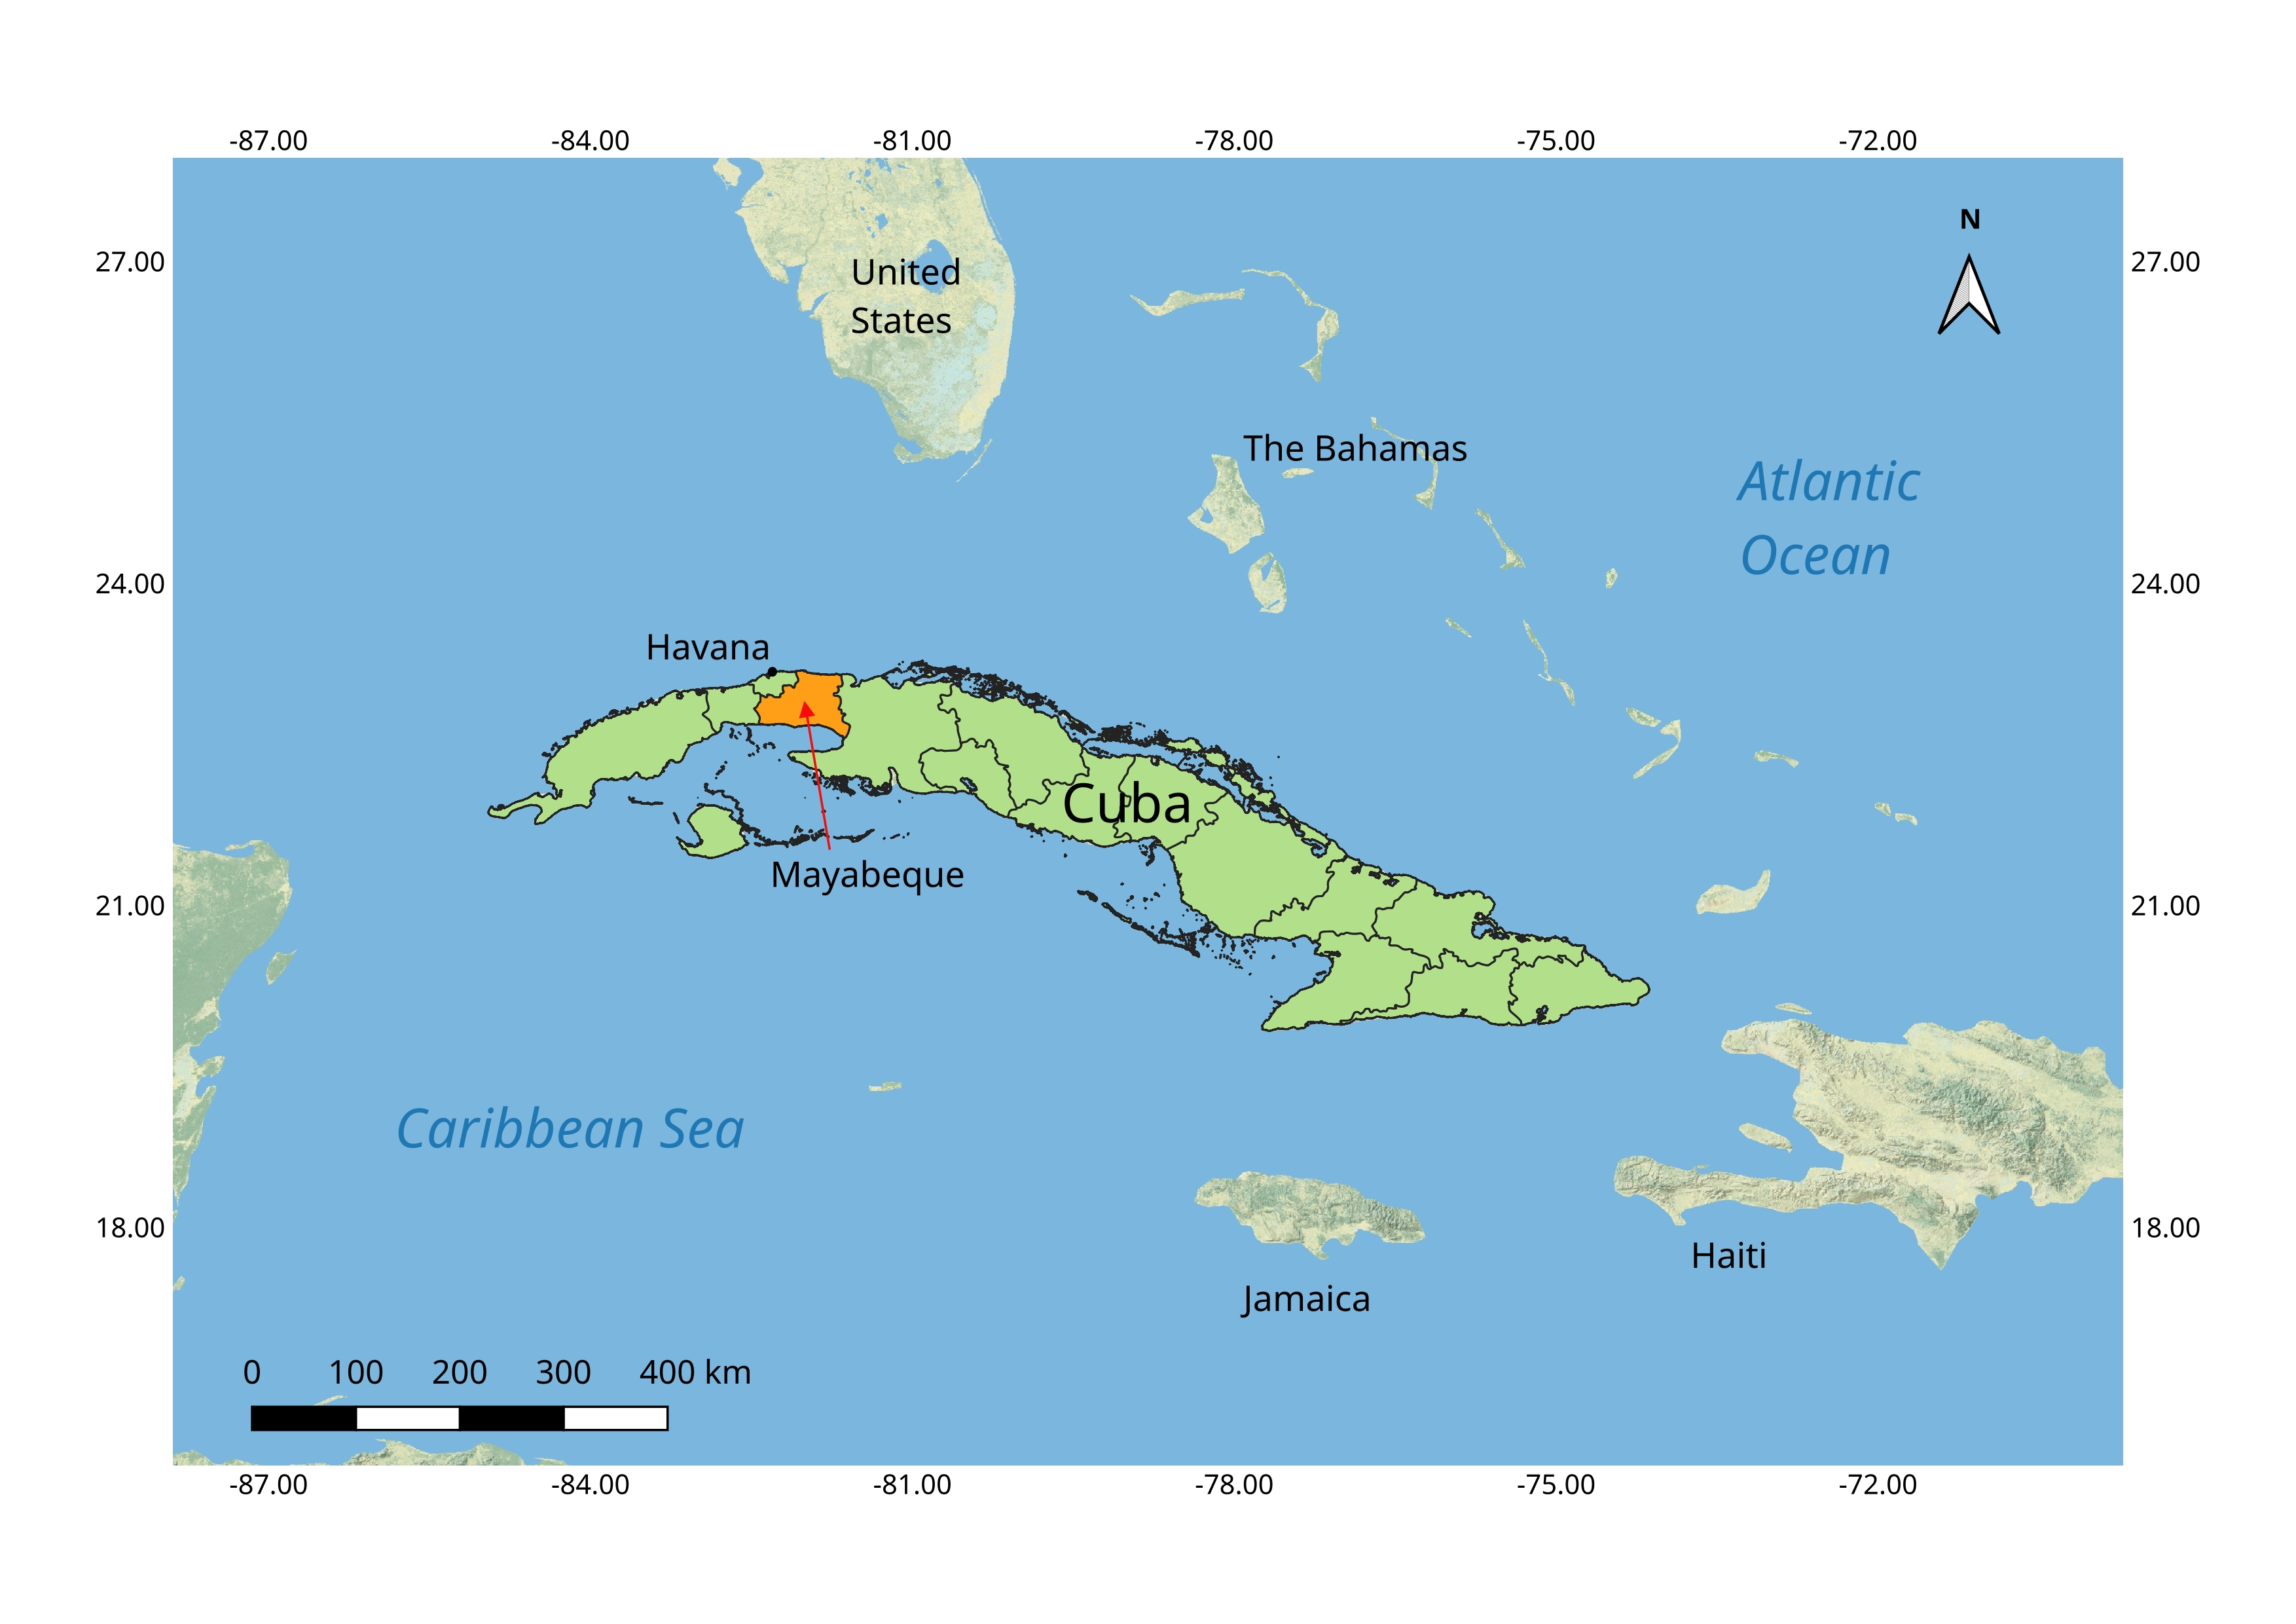
\includegraphics[
				width=\paperwidth,
				height=\paperheight
				]{caribe-cuba.jpg}
			};
			
			\fill[
			forest,
			opacity=0.86
			] (current page.south west)
			rectangle (current page.north east);
			
			\fill[
			gold
			] ([xshift=0.75cm,yshift=-1.35cm]current page.north west)
			rectangle
			([xshift=0.87cm,yshift=-5.85cm]current page.north west);
			
			\node[
			anchor=north west,
			align=left,
			text=white,
			text width=11.2cm
			] at ([xshift=1.2cm,yshift=-1.65cm]current page.north west) {
				
				{\color{mint}\large GEOSPATIAL ANALYSIS
					\hspace{0.3em}
					\textbullet
					\hspace{0.3em}
					REMOTE SENSING}
				
				\vspace{0.65cm}
				
				{\fontsize{35}{39}\selectfont
					\bfseries GeoSoil-Cuba}
				
				\vspace{0.45cm}
				
				{\fontsize{17}{22}\selectfont
					Integrating soil maps, land cover,
					and Sentinel-2 NDVI in Cuba}
				
				\vspace{1.0cm}
				
				{\large Ben Tamayo}
				
				\vspace{0.15cm}
				
				{\color{mint}\small
					Python \textbullet\ QGIS \textbullet\ GDAL
					\textbullet\ Rasterio \textbullet\ Sentinel-2}
				
				\vspace{0.7cm}
				
				{\color{white}\small October 2026}
			};
			
			\node[
			anchor=south east,
			text=white,
			align=right
			] at ([xshift=-0.7cm,yshift=0.45cm]current page.south east) {
				\scriptsize SOIL \textbullet\ VEGETATION \textbullet\ DATA
			};
			
		\end{tikzpicture}
		
	\end{frame}
	
	% ------------------------------------------------------------
	% 2. Project overview
	% ------------------------------------------------------------
	
	\begin{frame}{A GIS workflow built around a real landscape}
		
		\sectionlabel{The project}
		
		\begin{columns}[T,onlytextwidth]
			
			\column{0.56\textwidth}
			
			{\LARGE
				What can we learn by combining
				historical soil maps with
				satellite observations?
			}
			
			\vspace{0.45cm}
			
			\begin{itemize}
				\item Prepare historical soil cartography for contemporary GIS.
				\item Assess spatial coverage and geometric consistency.
				\item Integrate soil and vegetation information.
				\item Examine NDVI changes across an agricultural landscape.
			\end{itemize}
			
			\column{0.40\textwidth}
			
			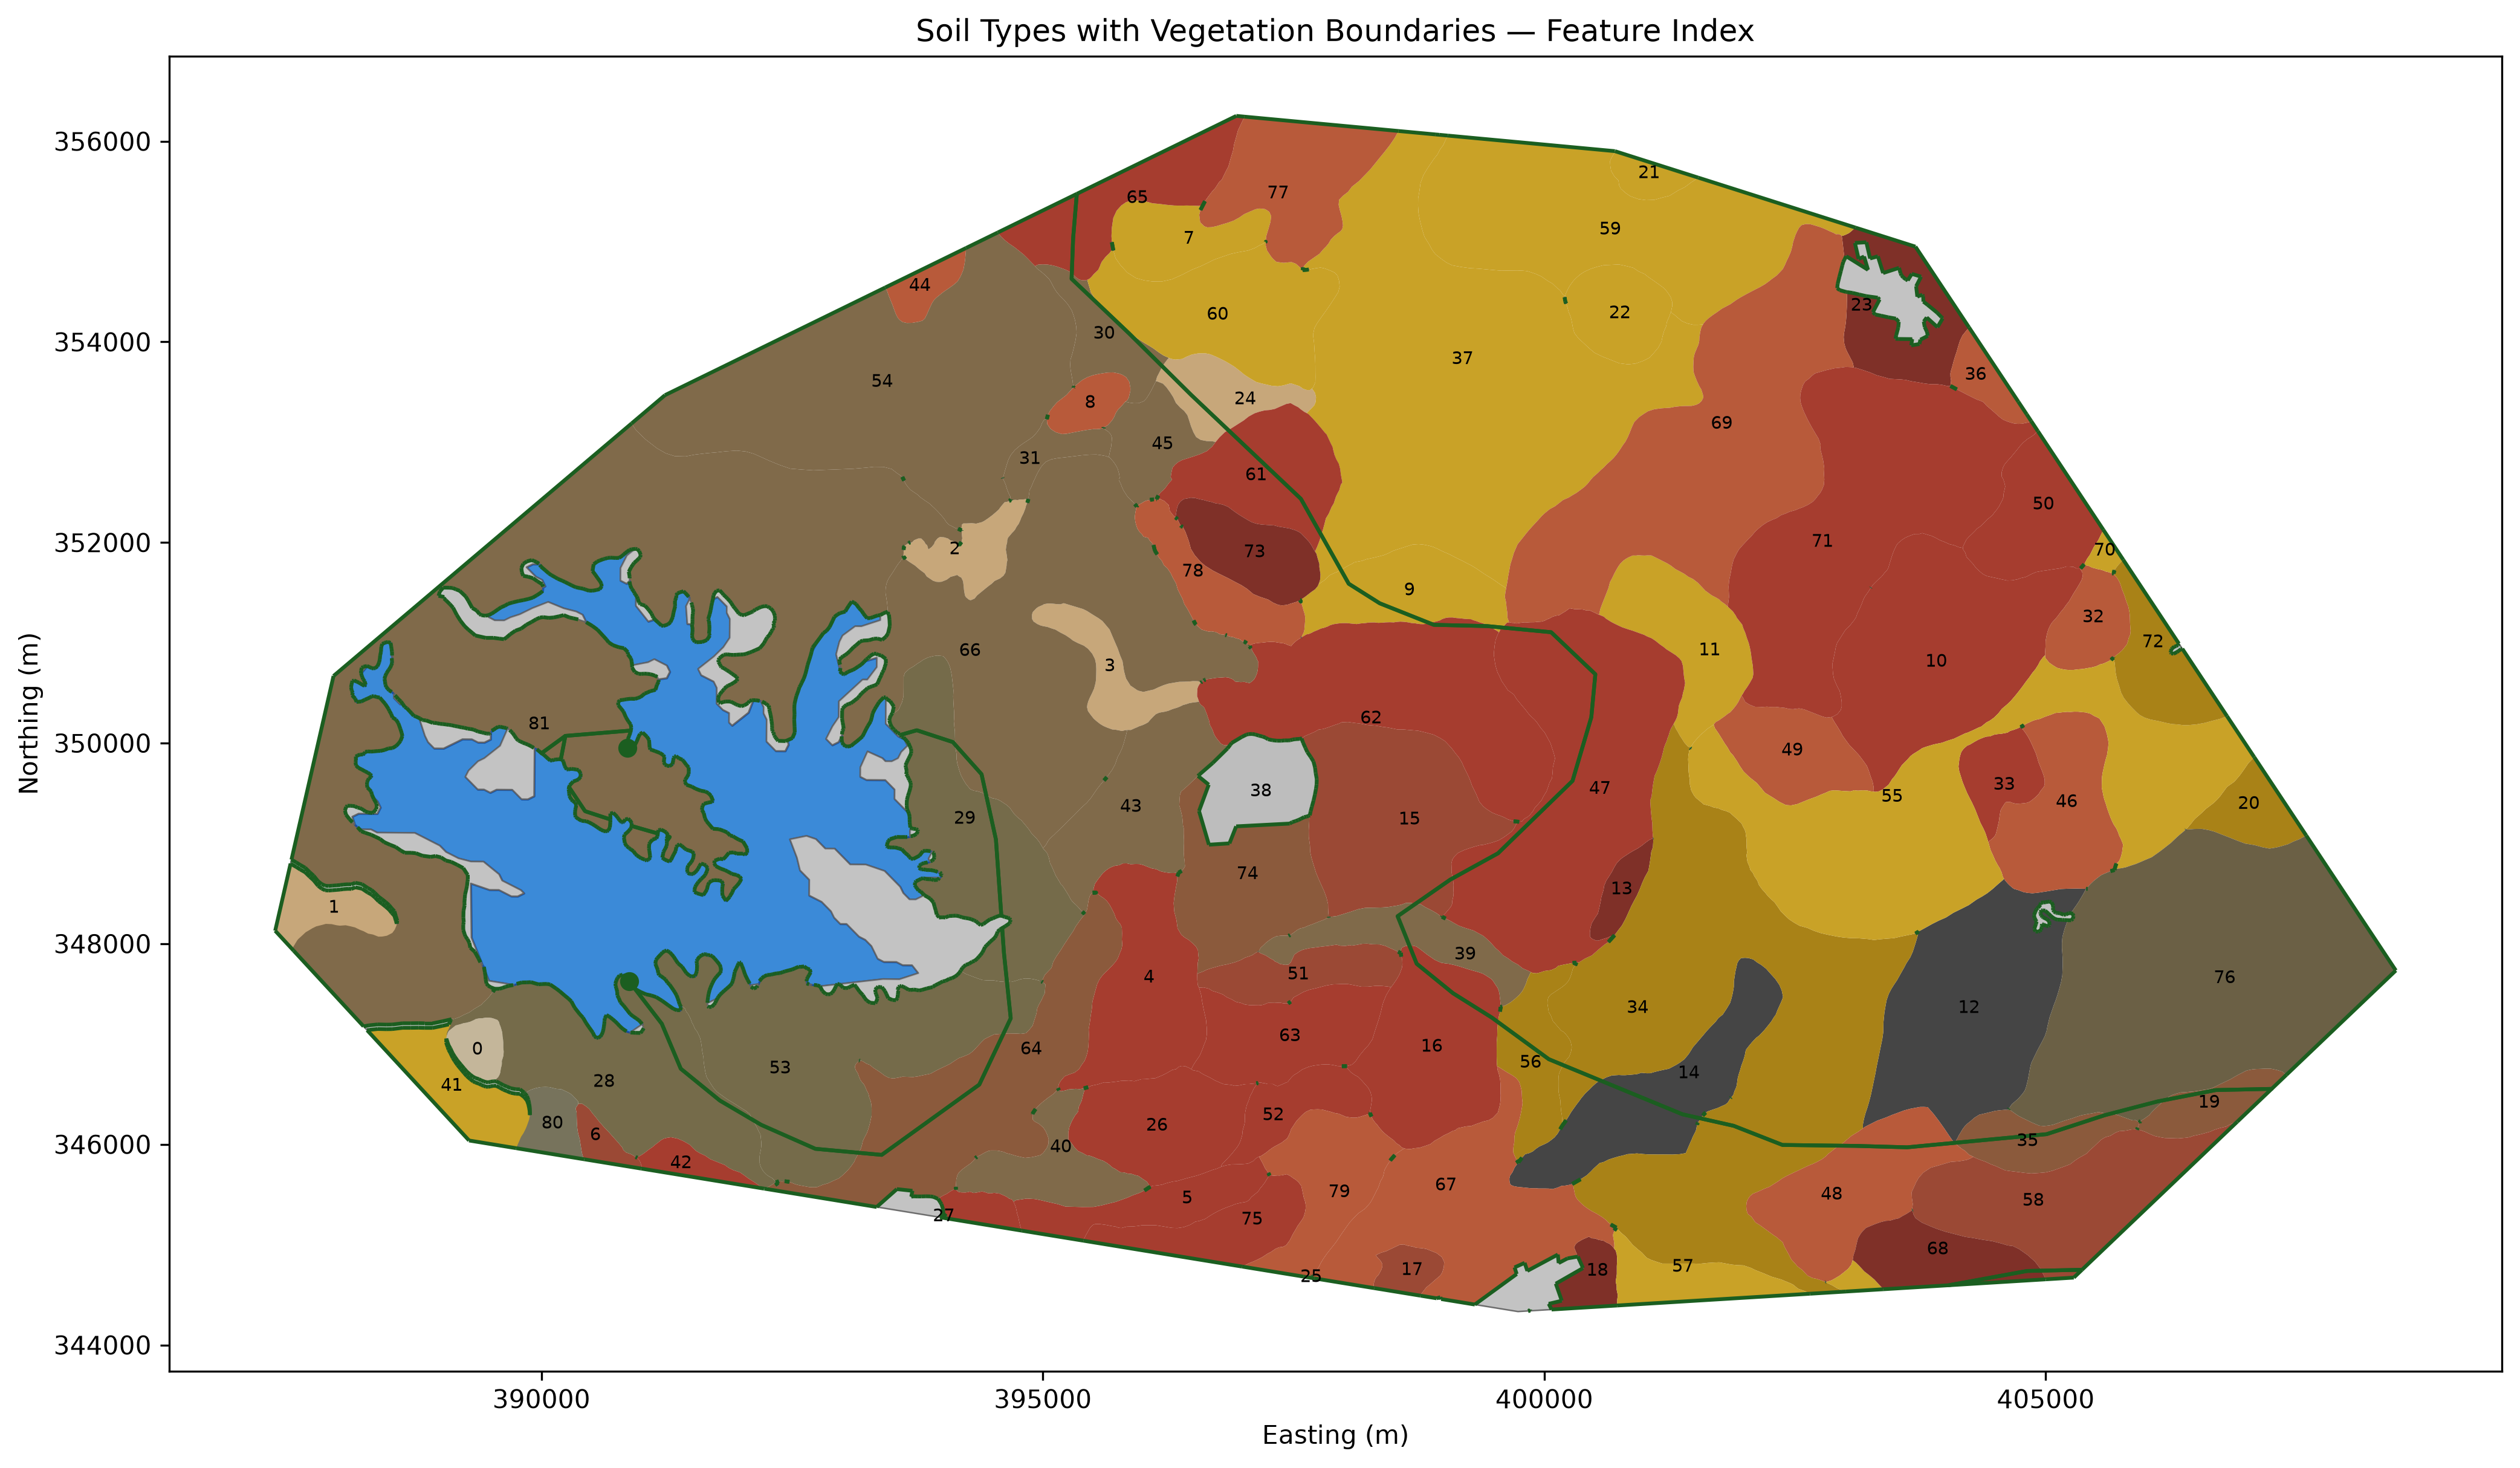
\includegraphics[
			width=\linewidth,
			height=5.2cm,
			keepaspectratio
			]{soil_types_with_vegetation_boundaries.png}
			
			\imagecaption{
				Soil units integrated with vegetation boundaries.
			}
			
		\end{columns}
		
		\takeaway{
			The project connects spatial-data quality assessment
			with satellite-based vegetation analysis.
		}
		
	\end{frame}
	
	% ------------------------------------------------------------
	% 3. Study area
	% ------------------------------------------------------------
	
	\begin{frame}{The study area: Jaruco, Mayabeque, Cuba}
		
		\begin{columns}[T,onlytextwidth]
			
			\column{0.61\textwidth}
			
			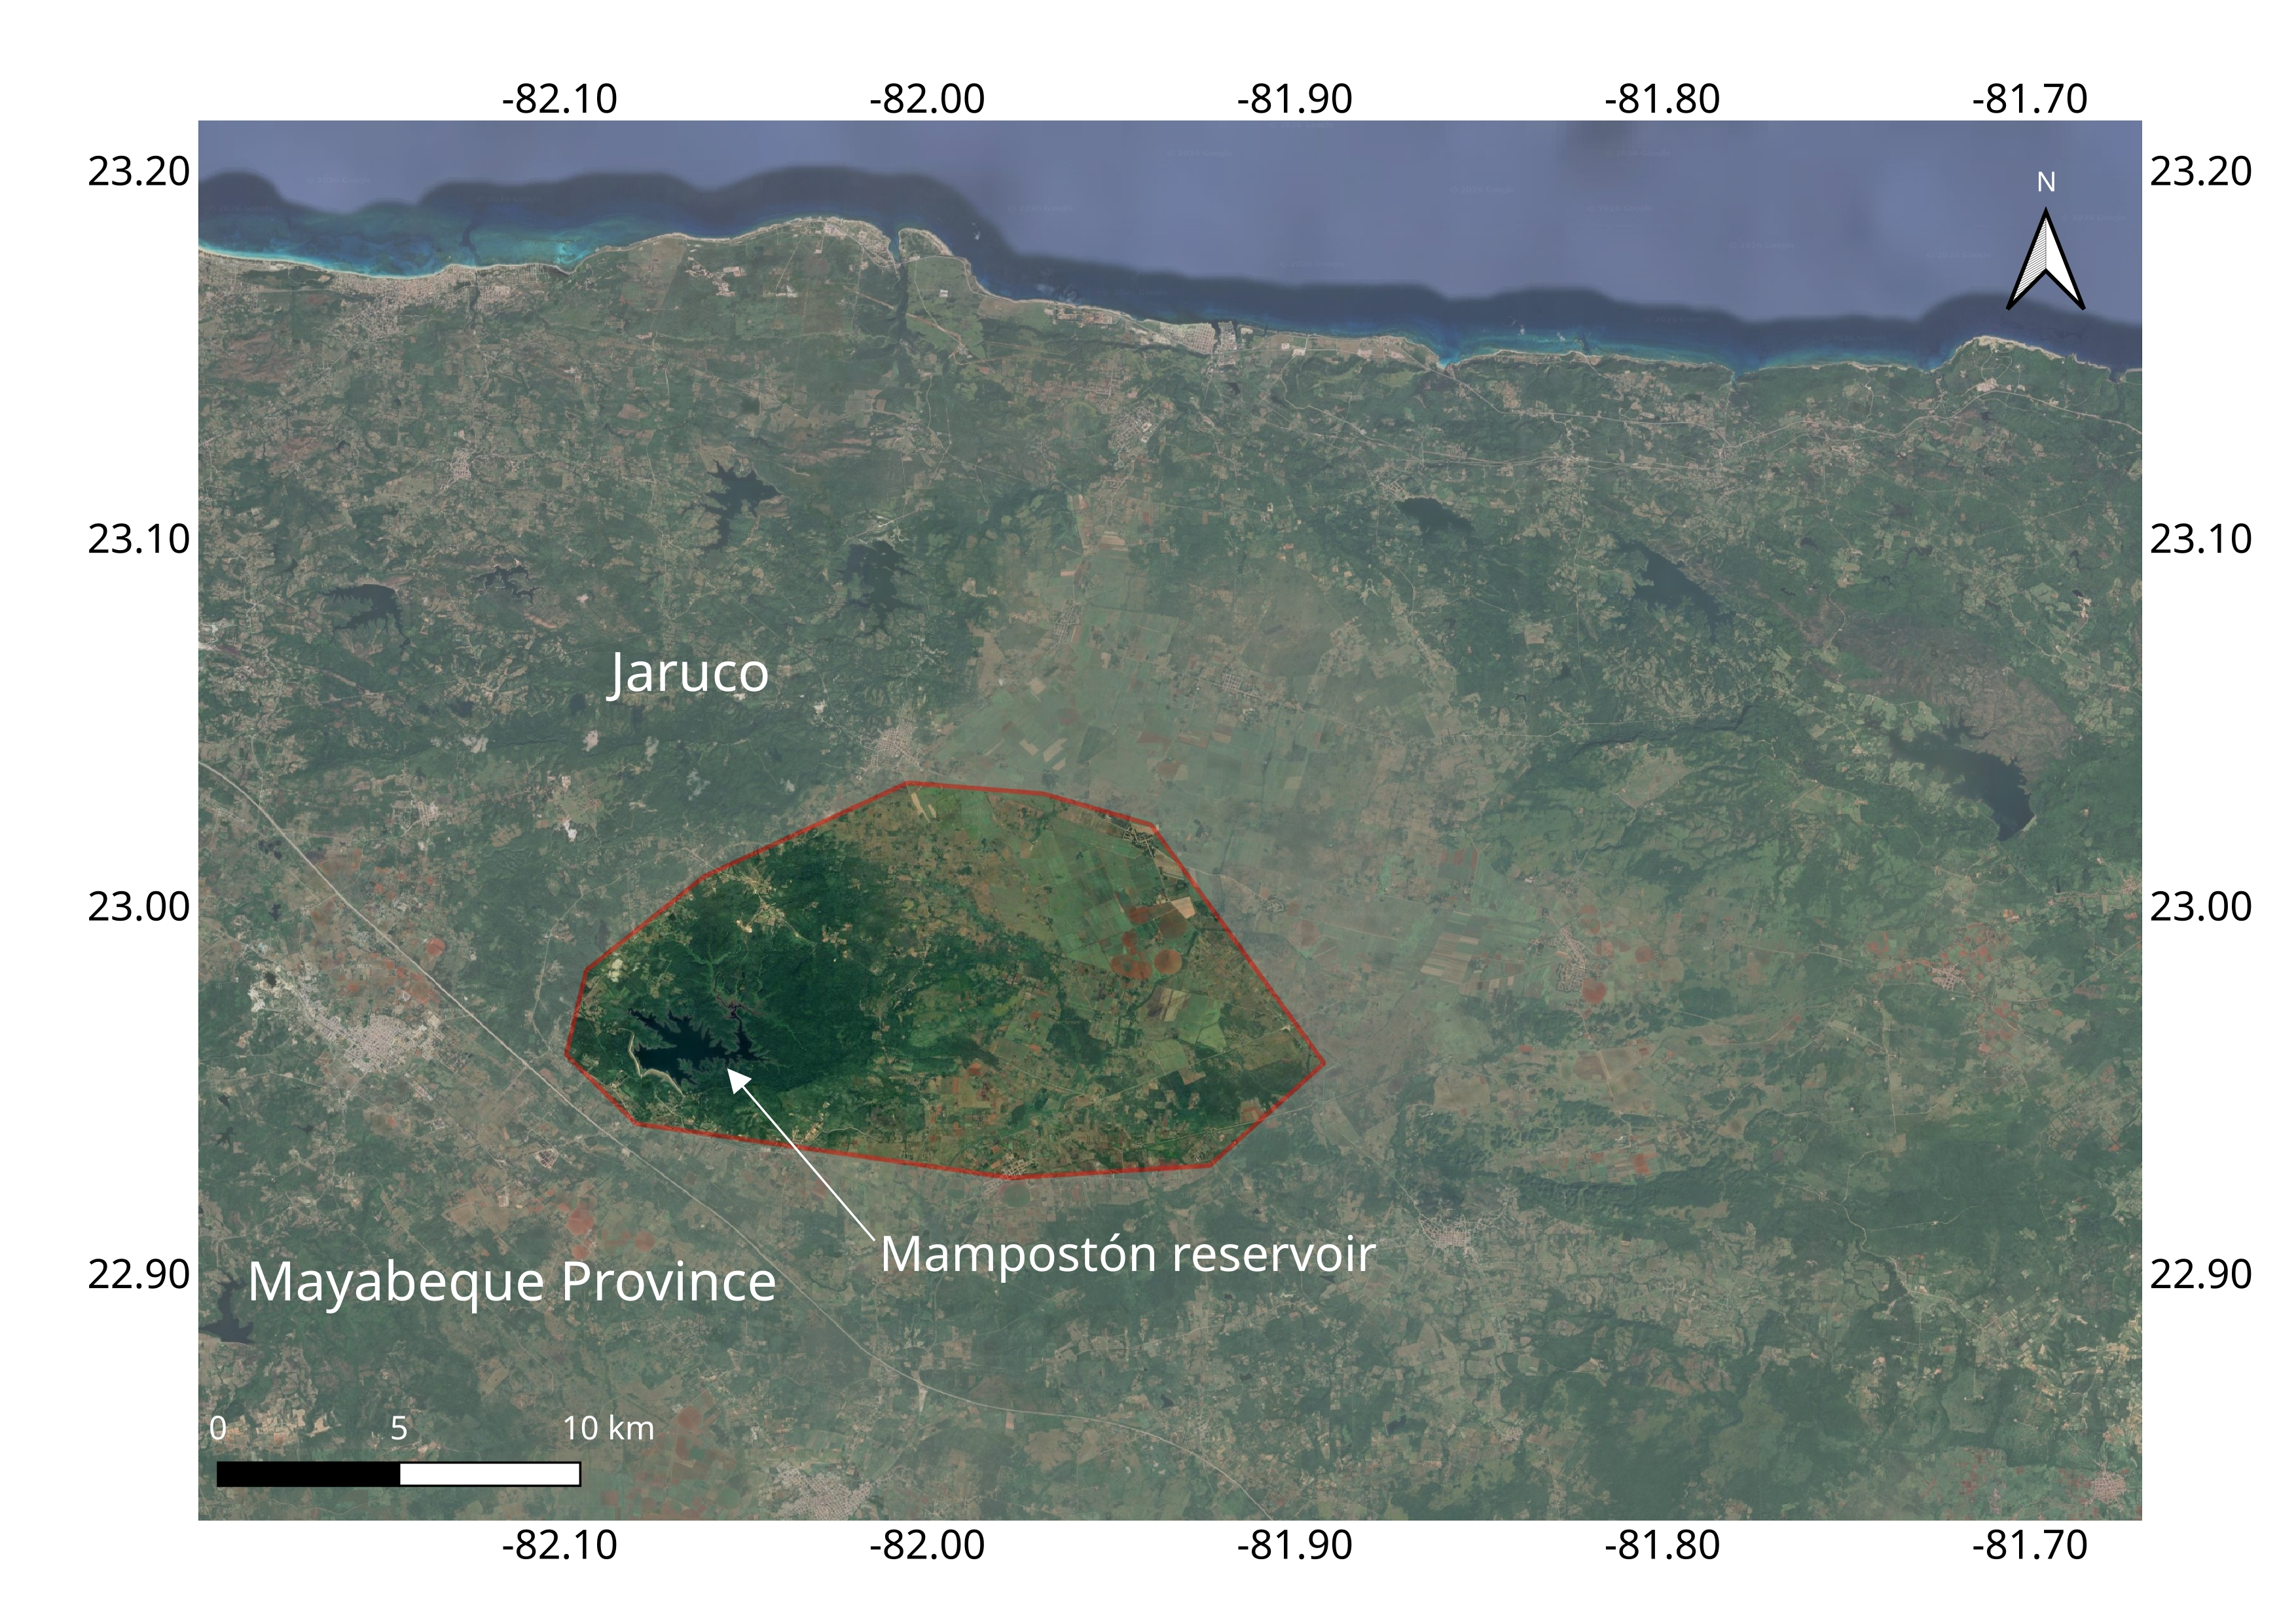
\includegraphics[
			width=\linewidth,
			height=5.5cm,
			keepaspectratio
			]{escala-mayabeque.jpg}
			
			\imagecaption{
				Geographic context and location of the study area.
			}
			
			\column{0.35\textwidth}
			
			\vspace{0.35cm}
			
			\metric{0.98\linewidth}{178.47 km$^2$}{Area of interest}
			
			\vspace{0.55cm}
			
			\metric{0.98\linewidth}{91.25\%}{Reported soil-map coverage}
			
			\vspace{0.55cm}
			
			\metric{0.98\linewidth}{3}{Selected potato-field samples}
			
		\end{columns}
		
		\vspace{0.25cm}
		
		\pill{Cuba Norte: EPSG:3795}
		\hspace{0.15cm}
		\pill{Satellite analysis: EPSG:32617}
		\hspace{0.15cm}
		\pill{QGIS + Python}
		
	\end{frame}
	
	% ------------------------------------------------------------
	% 4. Data and tools
	% ------------------------------------------------------------
	
	\begin{frame}{From historical maps to satellite imagery}
		
		\sectionlabel{Data and technology}
		
		\begin{columns}[T,onlytextwidth]
			
			\column{0.48\textwidth}
			
			\begin{beamercolorbox}[
				rounded=true,
				sep=0.25cm,
				wd=\linewidth
				]{block body}
				
				{\large\bfseries\color{forest}
					Historical soil cartography}
				
				\vspace{0.18cm}
				
				\small
				Soil polygons, soil classifications,
				water bodies, and source-map attributes.
				
				\vspace{0.25cm}
				
				\pill{Vector data}
				\hspace{0.1cm}
				\pill{GeoPackage}
				
			\end{beamercolorbox}
			
			\vspace{0.25cm}
			
			\begin{beamercolorbox}[
				rounded=true,
				sep=0.25cm,
				wd=\linewidth
				]{block body}
				
				{\large\bfseries\color{forest}
					Land cover and vegetation}
				
				\vspace{0.18cm}
				
				\small
				Vegetation boundaries and land-cover
				attributes for spatial integration.
				
				\vspace{0.25cm}
				
				\pill{Overlay}
				\hspace{0.1cm}
				\pill{Spatial analysis}
				
			\end{beamercolorbox}
			
			\column{0.48\textwidth}
			
			\begin{beamercolorbox}[
				rounded=true,
				sep=0.25cm,
				wd=\linewidth
				]{block body}
				
				{\large\bfseries\color{forest}
					Sentinel-2 Level-2A}
				
				\vspace{0.18cm}
				
				\small
				Red (B04), near-infrared (B08),
				and Scene Classification Layer (SCL).
				
				\vspace{0.25cm}
				
				\pill{10 m spectral bands}
				\hspace{0.1cm}
				\pill{NDVI}
				
			\end{beamercolorbox}
			
			\vspace{0.25cm}
			
			\begin{beamercolorbox}[
				rounded=true,
				sep=0.25cm,
				wd=\linewidth
				]{block body}
				
				{\large\bfseries\color{forest}
					Open-source tools}
				
				\vspace{0.18cm}
				
				\small
				Python, Jupyter, QGIS, GDAL,
				Rasterio, and pandas.
				
				\vspace{0.25cm}
				
				\pill{Reproducible workflow}
				
			\end{beamercolorbox}
			
		\end{columns}
		
	\end{frame}
	
	% ------------------------------------------------------------
	% 5. Workflow
	% ------------------------------------------------------------
	
	\begin{frame}{One workflow, two analytical scales}
		
		\sectionlabel{Methodology}
		
		\centering
		
		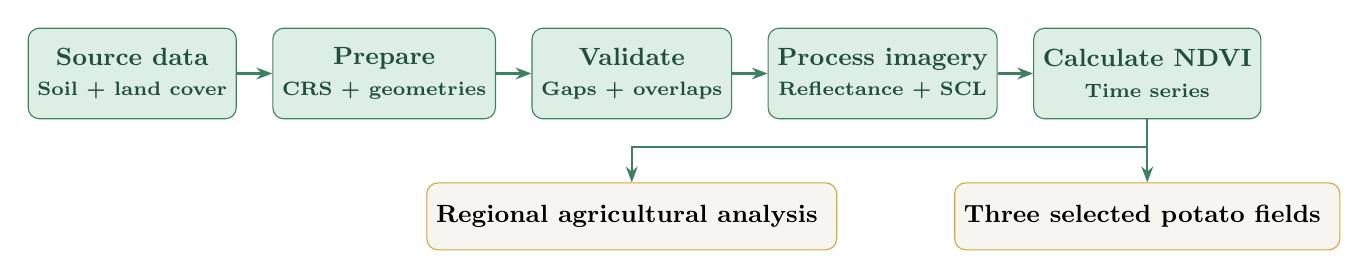
\begin{tikzpicture}[
			node distance=0.45cm,
			process/.style={
				rounded corners=4pt,
				draw=leaf,
				fill=mint,
				text=forest,
				align=center,
				minimum width=2.25cm,
				minimum height=1.15cm,
				font=\small\bfseries
			},
			arrow/.style={
				-{Stealth[length=2mm]},
				thick,
				draw=leaf
			}
			]
			
			\node[process] (source) {
				Source data\\
				\scriptsize Soil + land cover
			};
			
			\node[process,right=of source] (prepare) {
				Prepare\\
				\scriptsize CRS + geometries
			};
			
			\node[process,right=of prepare] (validate) {
				Validate\\
				\scriptsize Gaps + overlaps
			};
			
			\node[process,right=of validate] (satellite) {
				Process imagery\\
				\scriptsize Reflectance + SCL
			};
			
			\node[process,right=of satellite] (ndvi) {
				Calculate NDVI\\
				\scriptsize Time series
			};
			
			\draw[arrow] (source) -- (prepare);
			\draw[arrow] (prepare) -- (validate);
			\draw[arrow] (validate) -- (satellite);
			\draw[arrow] (satellite) -- (ndvi);
			
			\node[
			below=0.8cm of validate,
			rounded corners=4pt,
			fill=cream,
			draw=gold,
			minimum width=4.5cm,
			minimum height=0.85cm,
			align=center,
			font=\small\bfseries
			] (regional) {
				Regional agricultural analysis
			};
			
			\node[
			below=0.8cm of ndvi,
			rounded corners=4pt,
			fill=cream,
			draw=gold,
			minimum width=4.5cm,
			minimum height=0.85cm,
			align=center,
			font=\small\bfseries
			] (field) {
				Three selected potato fields
			};
			
			\draw[arrow] (ndvi.south) -- ++(0,-0.35) -| (regional.north);
			\draw[arrow] (ndvi.south) -- ++(0,-0.35) -| (field.north);
			
		\end{tikzpicture}
		
		\vspace{0.5cm}
		
		\begin{columns}[T,onlytextwidth]
			
			\column{0.48\textwidth}
			
			\textbf{\color{forest}Spatial data quality}
			
			\small
			Geometry validity, coverage, coordinate
			reference systems, and overlap assessment.
			
			\column{0.48\textwidth}
			
			\textbf{\color{forest}Vegetation dynamics}
			
			\small
			Cloud screening, raster calculations,
			temporal statistics, and field comparisons.
			
		\end{columns}
		
	\end{frame}
	
	% ------------------------------------------------------------
	% 6. Soil mapping
	% ------------------------------------------------------------
	
	\begin{frame}{Preparing soil cartography for spatial analysis}
		
		\begin{columns}[T,onlytextwidth]
			
			\column{0.60\textwidth}
			
			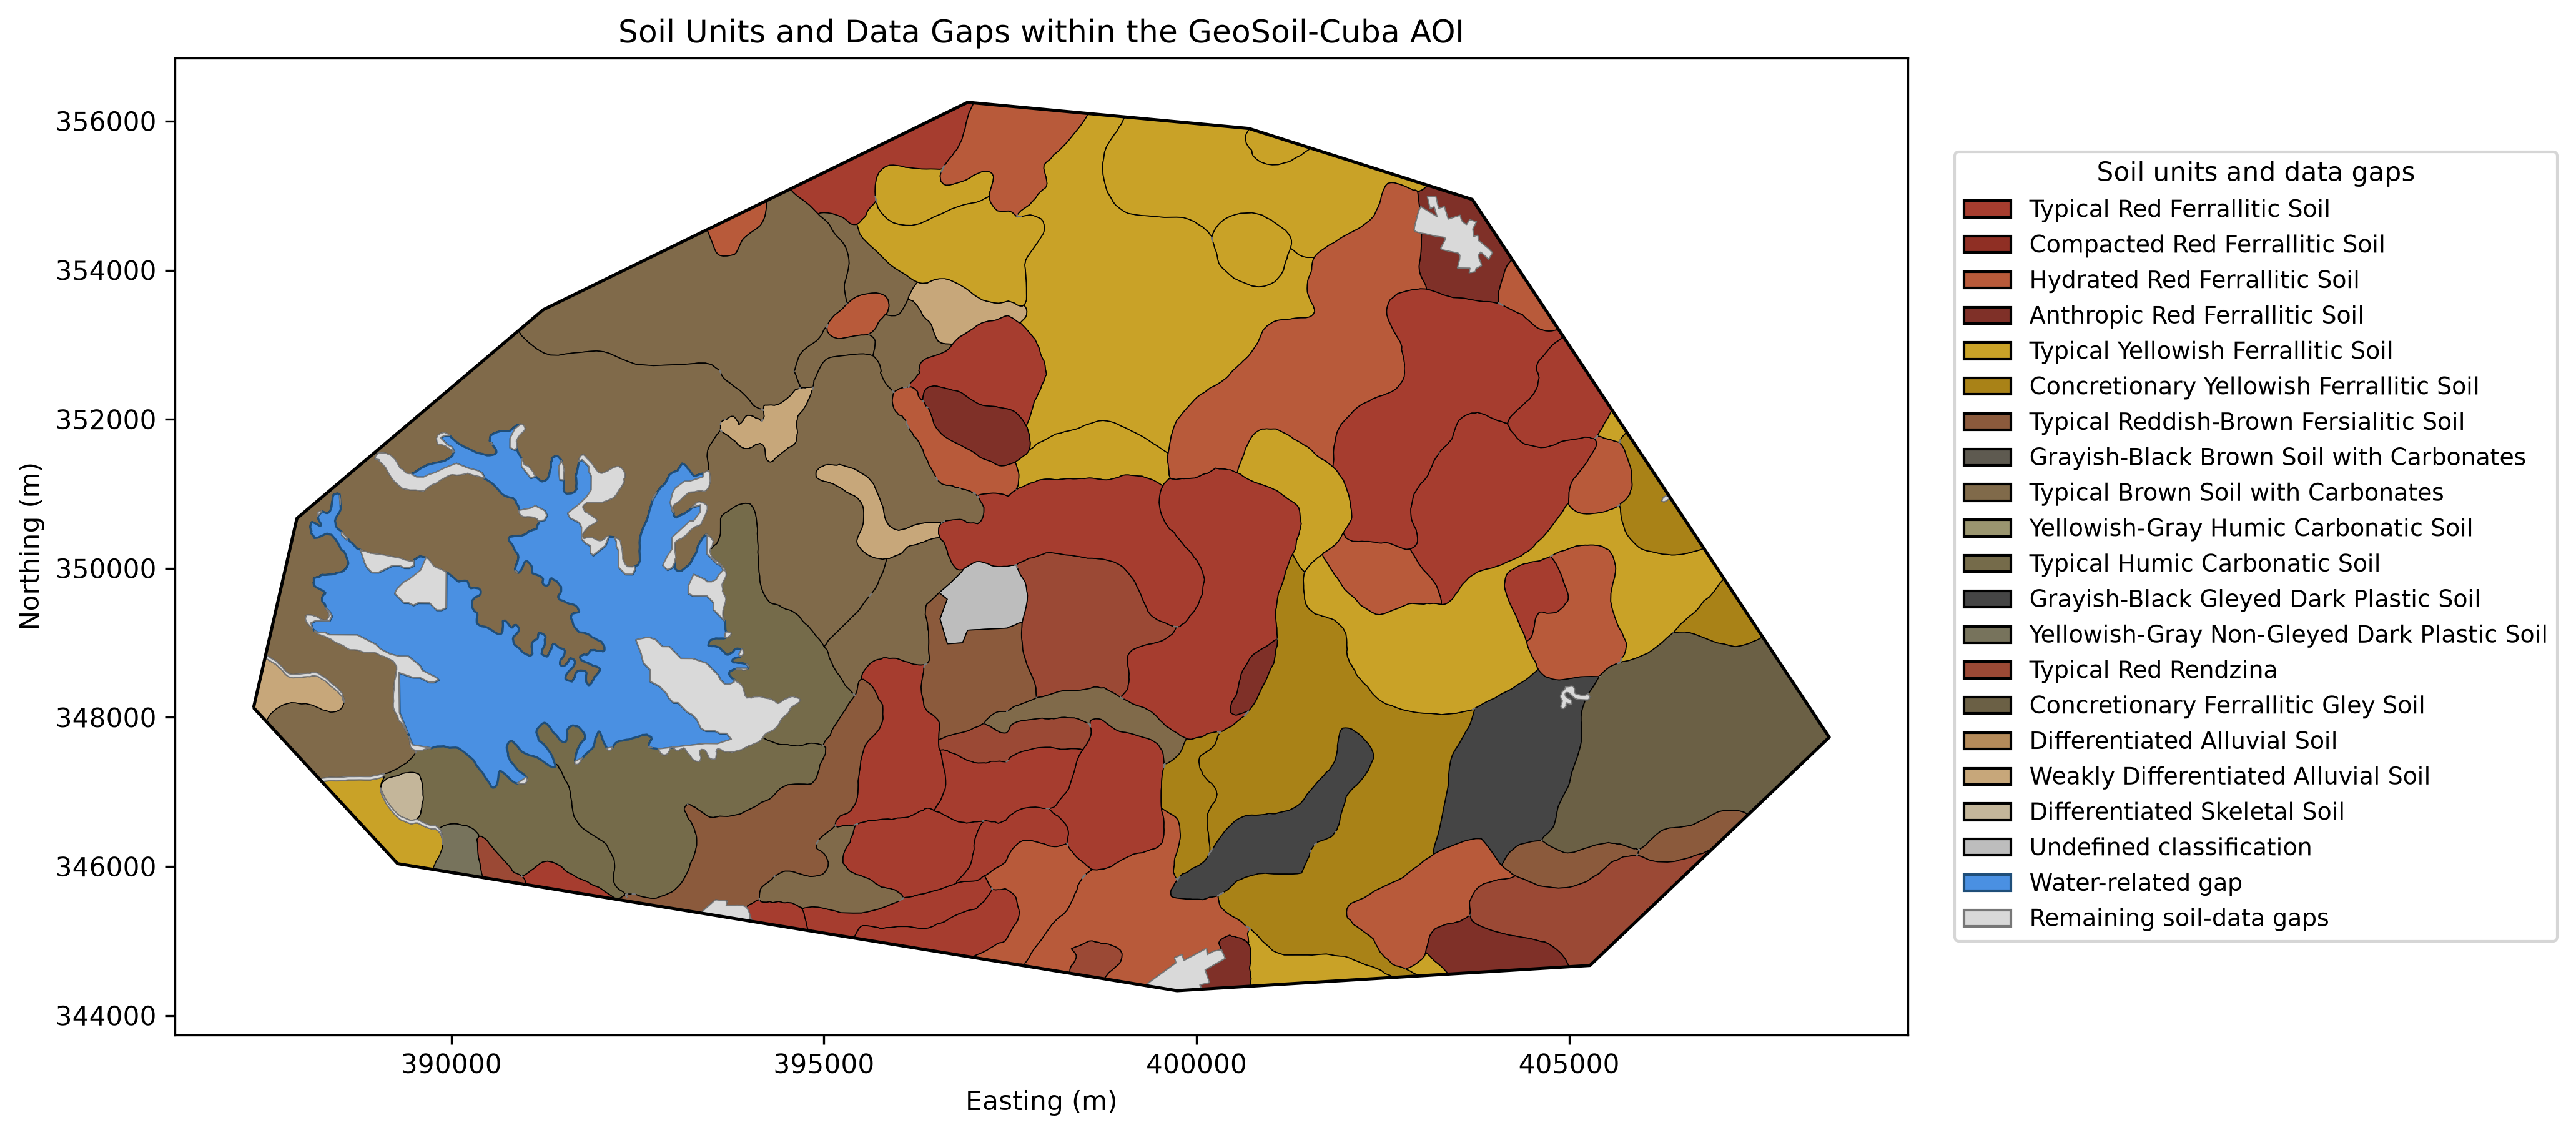
\includegraphics[
			width=\linewidth,
			height=5.6cm,
			keepaspectratio
			]{soil_units_aoi.png}
			
			\imagecaption{
				Soil units clipped to the area of interest.
			}
			
			\column{0.36\textwidth}
			
			\sectionlabel{Why preparation matters}
			
			{\large\bfseries
				A map is more than its polygons.
			}
			
			\vspace{0.25cm}
			
			\begin{itemize}
				\item Harmonize coordinate reference systems.
				\item Inspect geometry validity.
				\item Evaluate spatial coverage.
				\item Preserve source attributes.
				\item Check the consistency of polygon areas.
			\end{itemize}
			
		\end{columns}
		
		\takeaway{
			Spatial analysis depends on understanding the
			quality and limitations of its input data.
		}
		
	\end{frame}
	
	% ------------------------------------------------------------
	% 7. Coverage results
	% ------------------------------------------------------------
	
	\begin{frame}{How complete is the soil map?}
		
		\begin{columns}[T,onlytextwidth]
			
			\column{0.56\textwidth}
			
			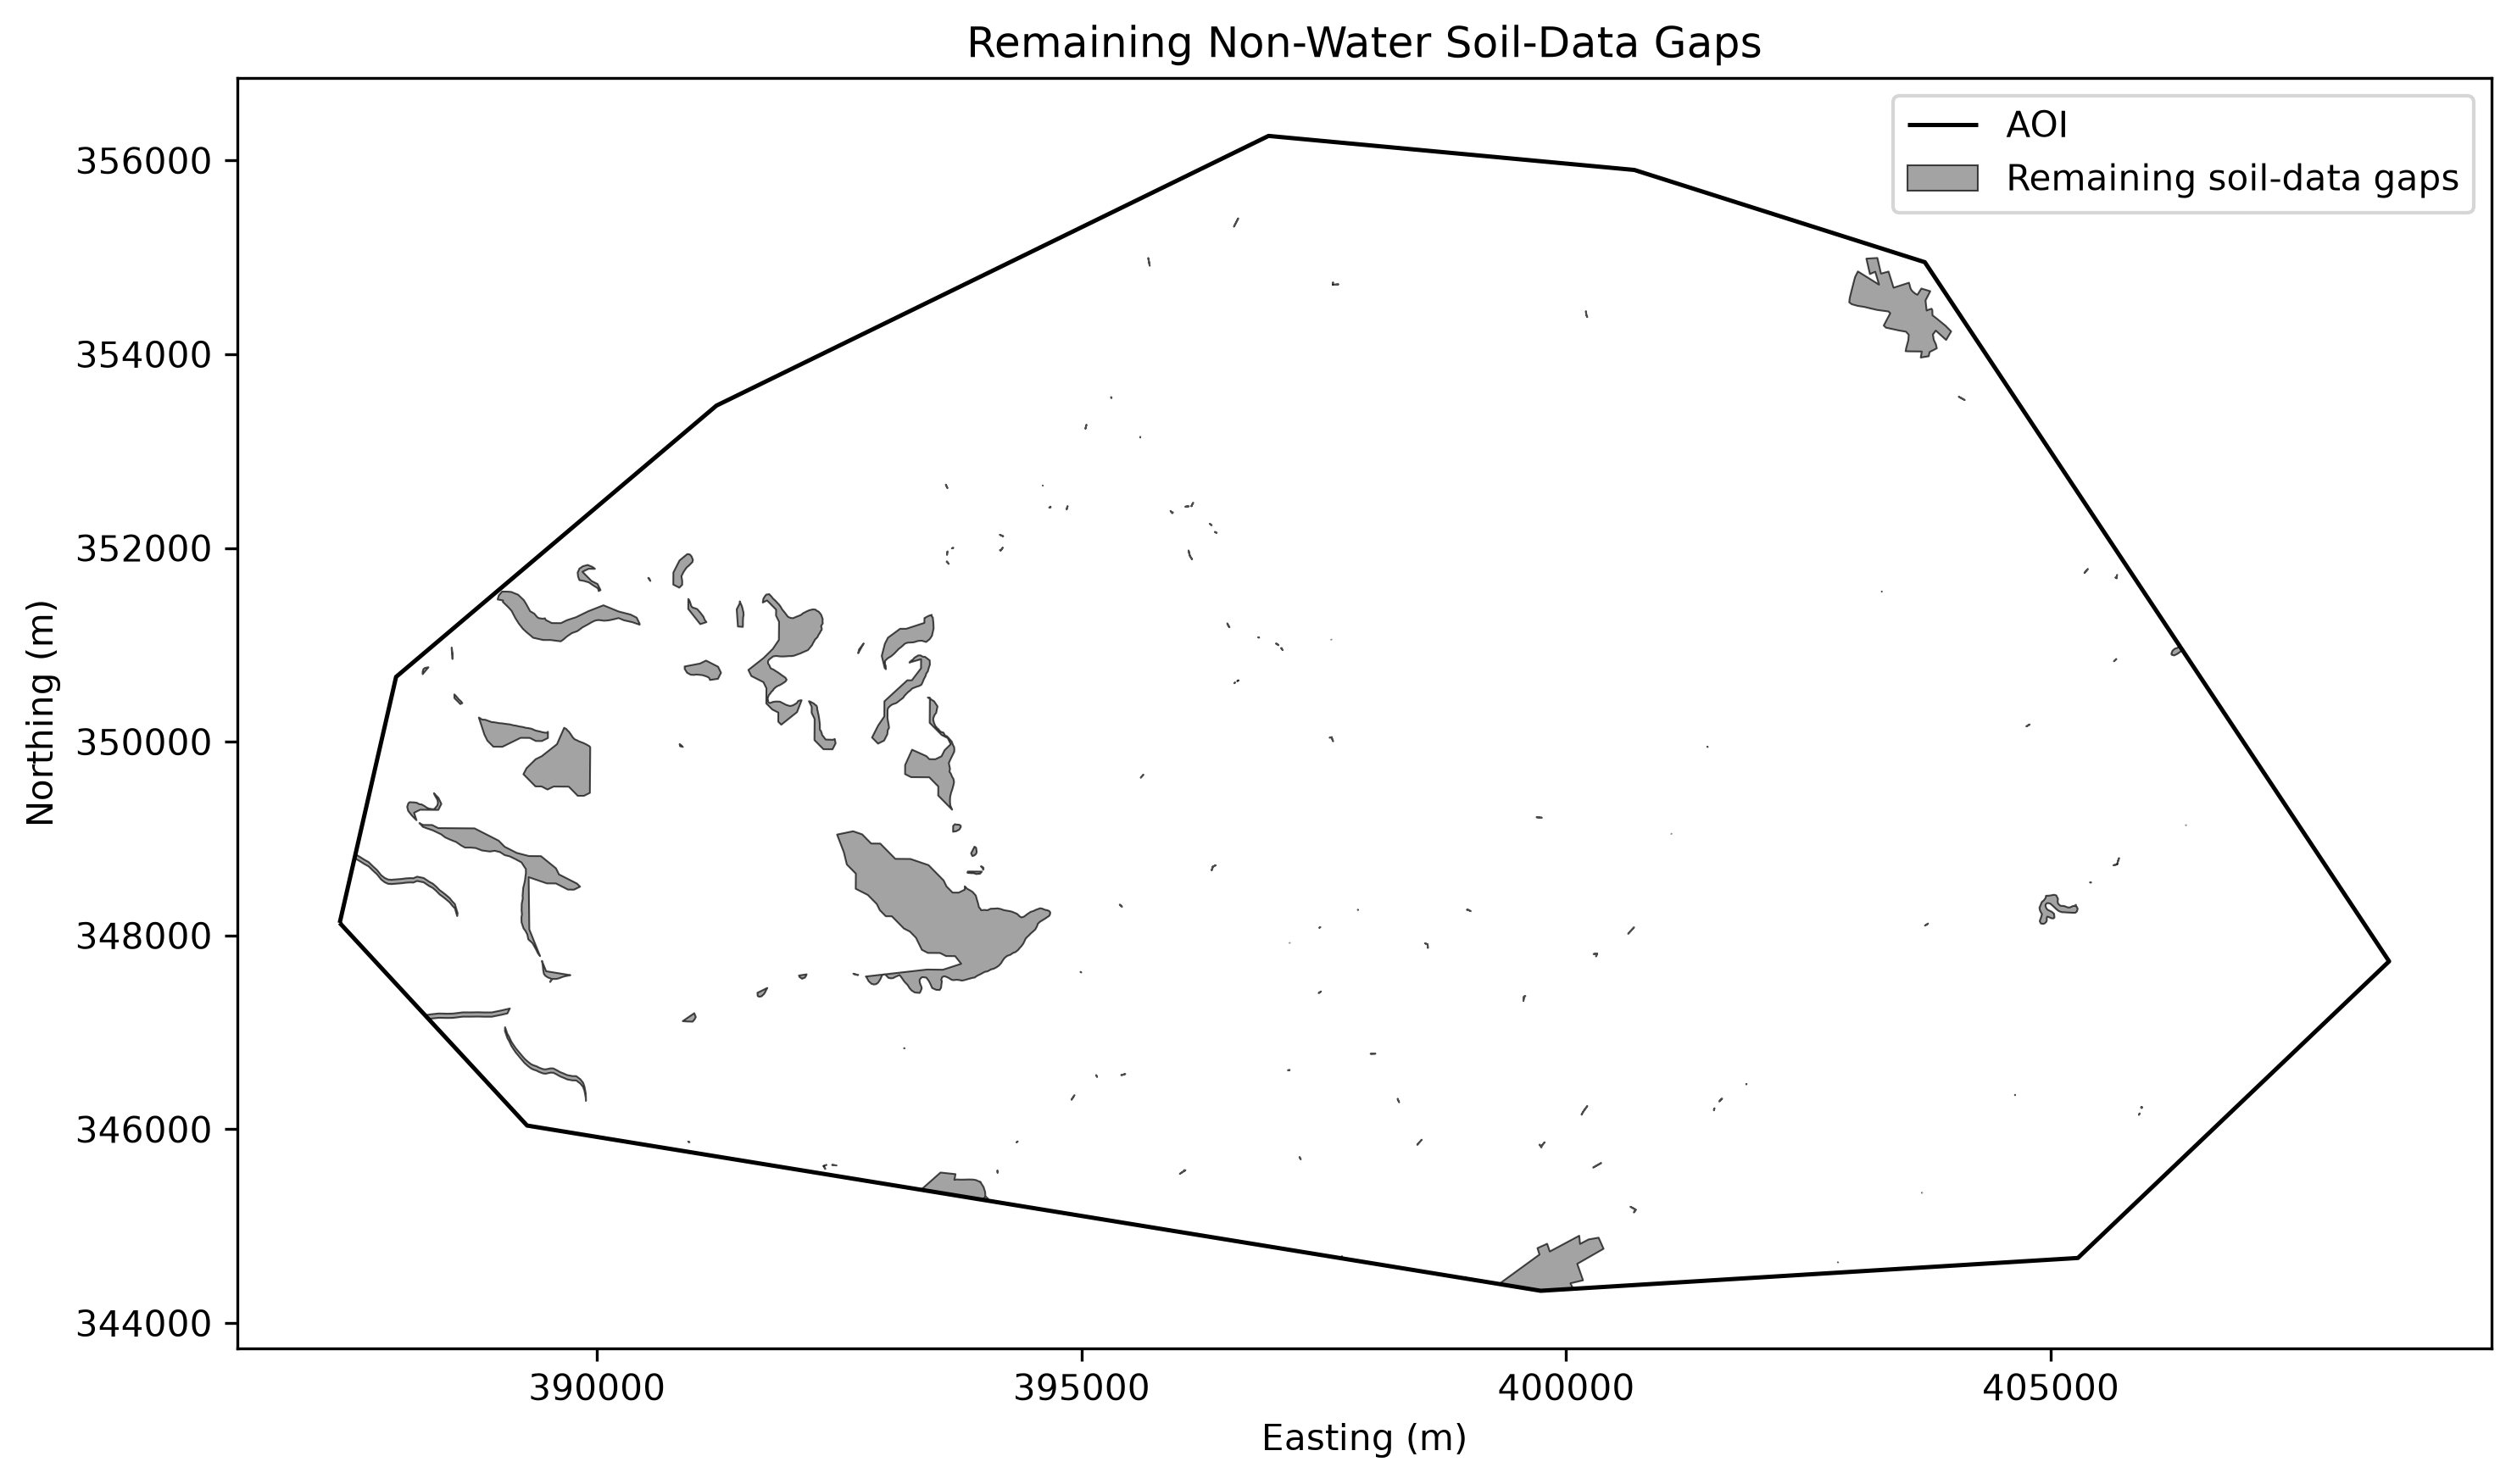
\includegraphics[
			width=\linewidth,
			height=5.4cm,
			keepaspectratio
			]{remaining_soil_data_gaps.png}
			
			\imagecaption{
				Spatial distribution of the remaining soil-data gaps.
			}
			
			\column{0.40\textwidth}
			
			\metric{0.98\linewidth}{178.47 km$^2$}{Total AOI}
			
			\vspace{0.35cm}
			
			\metric{0.98\linewidth}{162.85 km$^2$}{Reported soil-map coverage}
			
			\vspace{0.35cm}
			
			\metric{0.98\linewidth}{4.20 km$^2$}{Remaining non-water gaps}
			
			\vspace{0.25cm}
			
			\begin{beamercolorbox}[
				rounded=true,
				sep=0.18cm,
				wd=\linewidth
				]{block body}
				
				\small
				Remaining non-water gaps represent
				approximately \textbf{2.35\%} of the AOI.
				
			\end{beamercolorbox}
			
		\end{columns}
		
	\end{frame}
	
	% ------------------------------------------------------------
	% 8. Topology assessment
	% ------------------------------------------------------------
	
	\begin{frame}{Geometry checks reveal hidden spatial issues}
		
		\begin{columns}[T,onlytextwidth]
			
			\column{0.55\textwidth}
			
			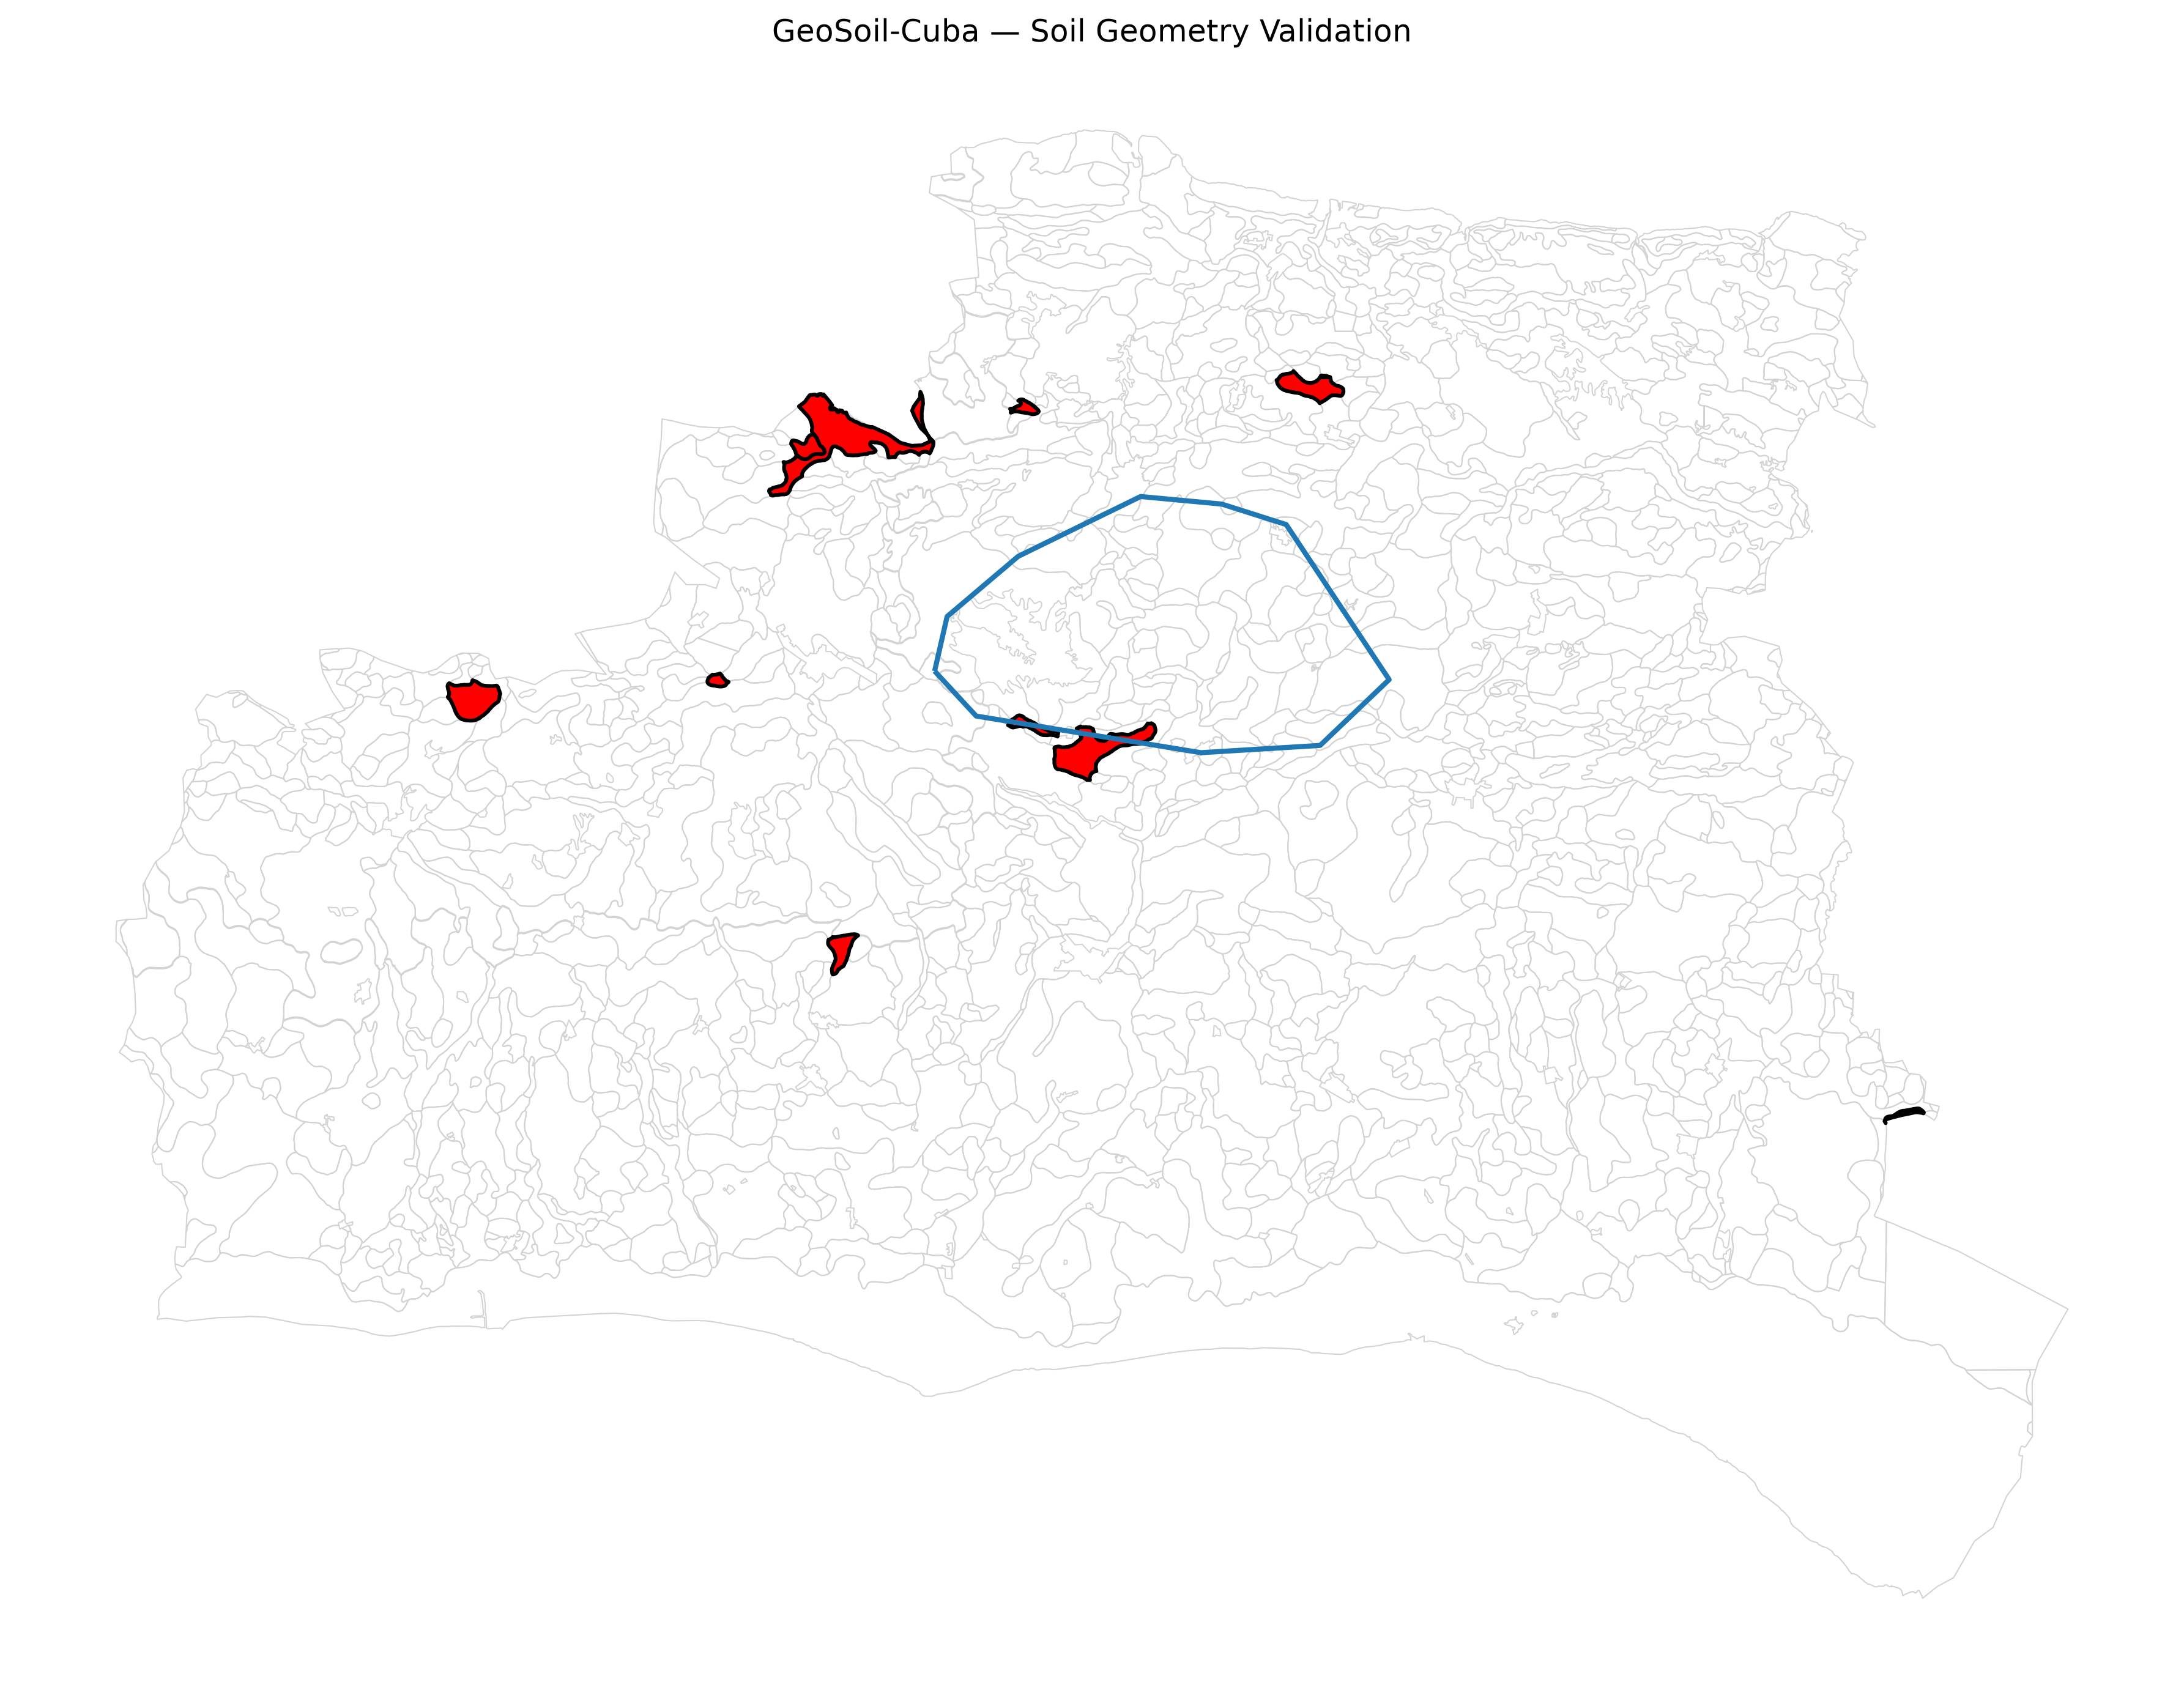
\includegraphics[
			width=\linewidth,
			height=5.3cm,
			keepaspectratio
			]{invalid_geometries.png}
			
			\imagecaption{
				Geometry inspection and spatial-data validation.
			}
			
			\column{0.41\textwidth}
			
			\sectionlabel{Topology results}
			
			\metric{0.98\linewidth}{90}{Polygon pairs with positive-area overlaps}
			
			\vspace{0.4cm}
			
			\metric{0.98\linewidth}{0.054919 km$^2$}{Cumulative pairwise overlap area}
			
			\vspace{0.4cm}
			
			\metric{0.98\linewidth}{0.046807 km$^2$}{Largest reported individual overlap}
			
		\end{columns}
		
		\takeaway{
			Area sums and geometric unions help identify
			overlaps that should be investigated before interpretation.
		}
		
	\end{frame}
	
	% ------------------------------------------------------------
	% 9. Sentinel-2 and NDVI
	% ------------------------------------------------------------
	
	\begin{frame}{Turning satellite reflectance into NDVI}
		
		\begin{columns}[T,onlytextwidth]
			
			\column{0.48\textwidth}
			
			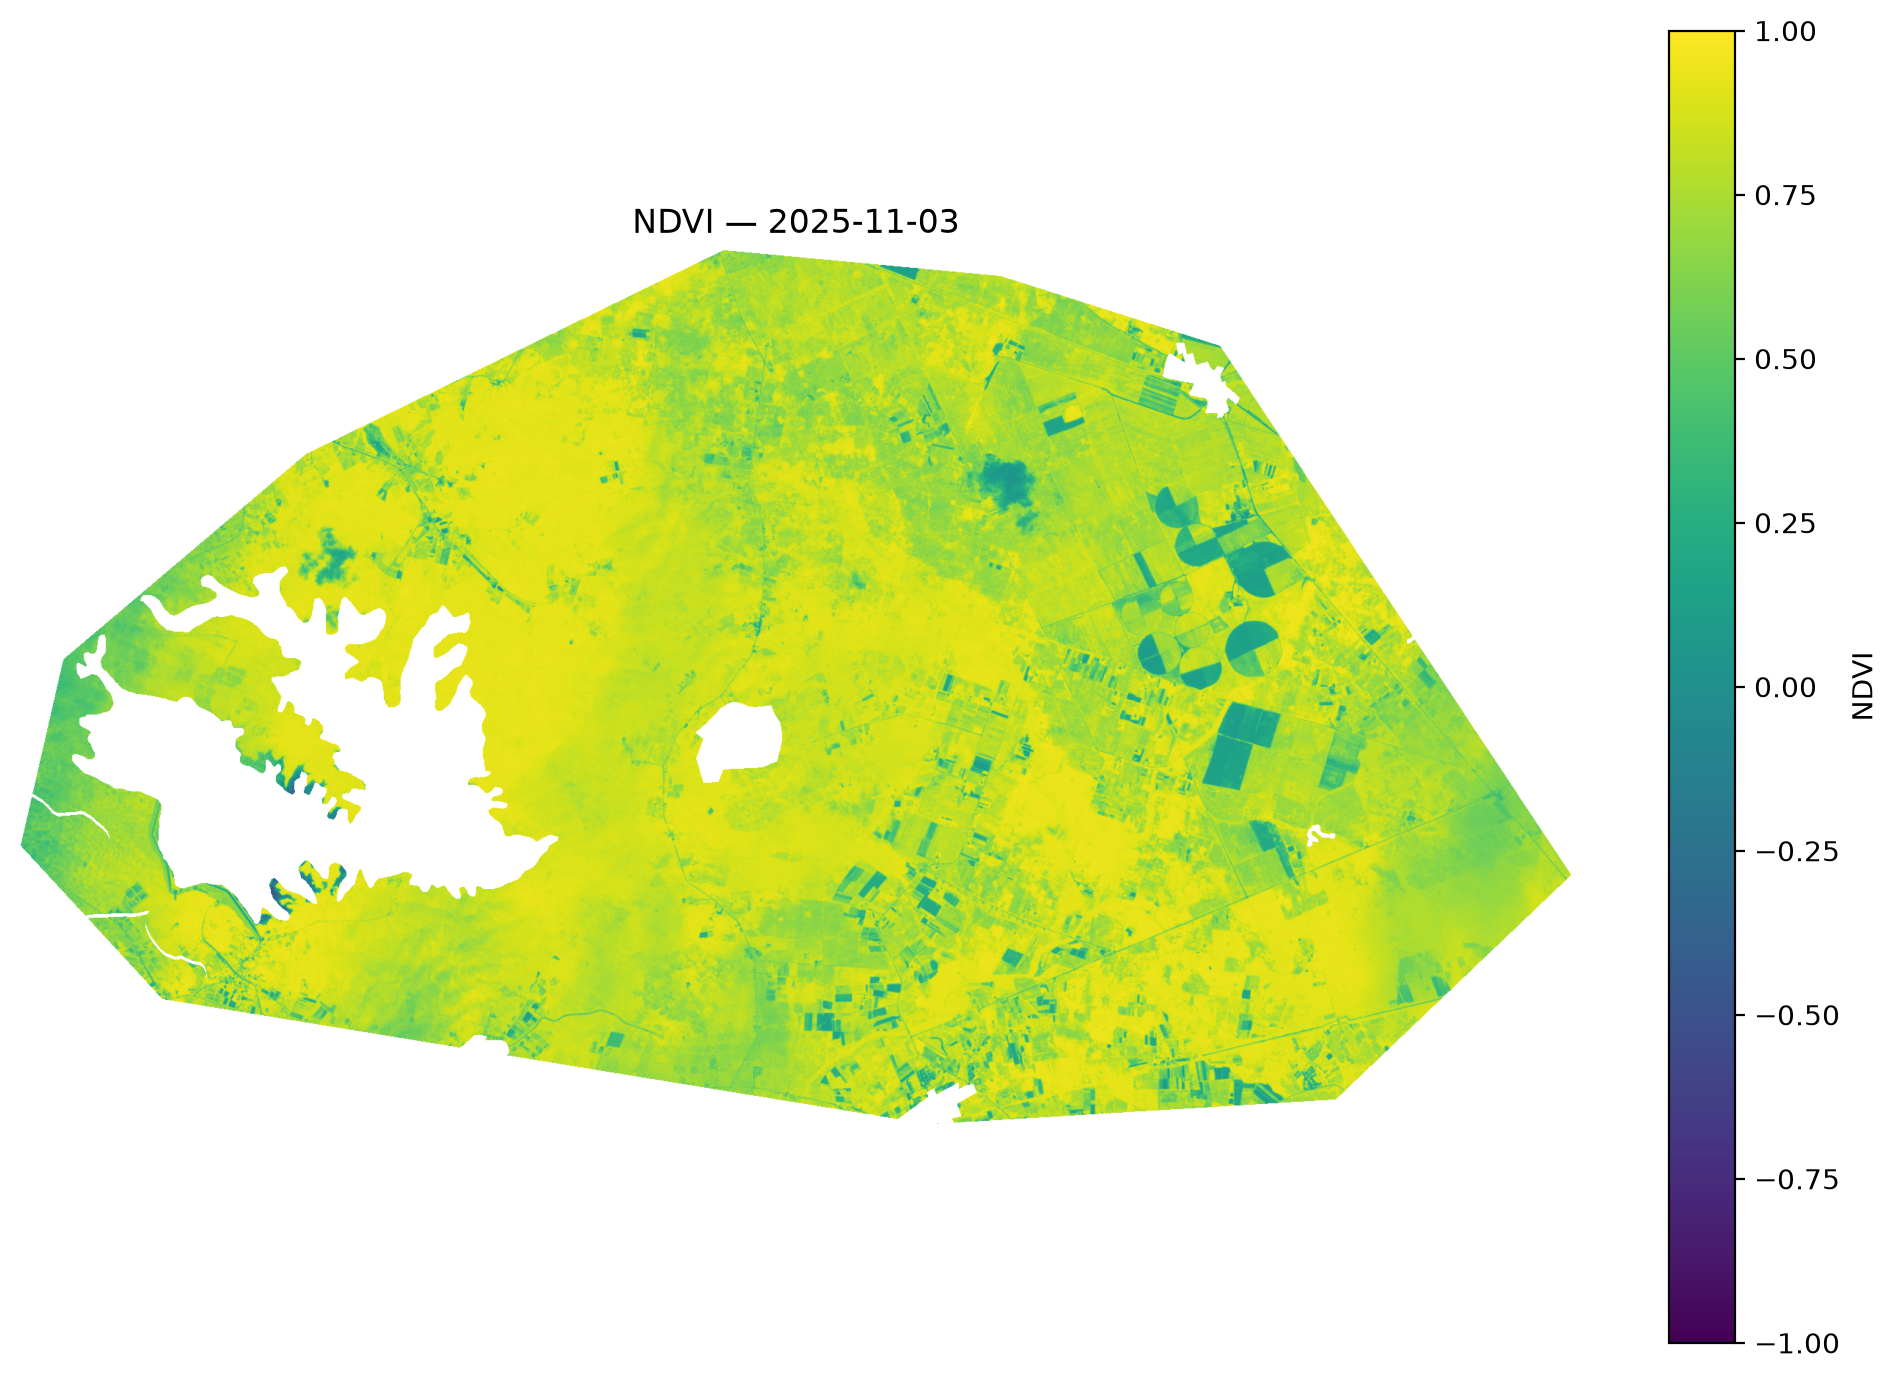
\includegraphics[
			width=\linewidth,
			height=4.6cm,
			keepaspectratio
			]{stage5_figure_23.png}
			
			\imagecaption{
				Example of the project's regional NDVI processing.
			}
			
			\column{0.48\textwidth}
			
			\sectionlabel{Normalized Difference Vegetation Index}
			
			\[
			\mathrm{NDVI} =
			\frac{
				\rho_{\mathrm{B08}}-\rho_{\mathrm{B04}}
			}{
				\rho_{\mathrm{B08}}+\rho_{\mathrm{B04}}
			}
			\]
			
			\vspace{0.2cm}
			
			\small
			
			\textbf{B08:} Near-infrared reflectance
			
			\textbf{B04:} Red reflectance
			
			\vspace{0.35cm}
			
			\begin{beamercolorbox}[
				rounded=true,
				sep=0.2cm,
				wd=\linewidth
				]{block body}
				
				\small
				Higher NDVI values generally indicate
				stronger vegetation greenness, but NDVI
				is not a direct measure of crop yield.
				
			\end{beamercolorbox}
			
		\end{columns}
		
	\end{frame}
	
	% ------------------------------------------------------------
	% 10. Image inventory and screening
	% ------------------------------------------------------------
	
	\begin{frame}{Screening satellite observations}
		
		\begin{columns}[T,onlytextwidth]
			
			\column{0.59\textwidth}
			
			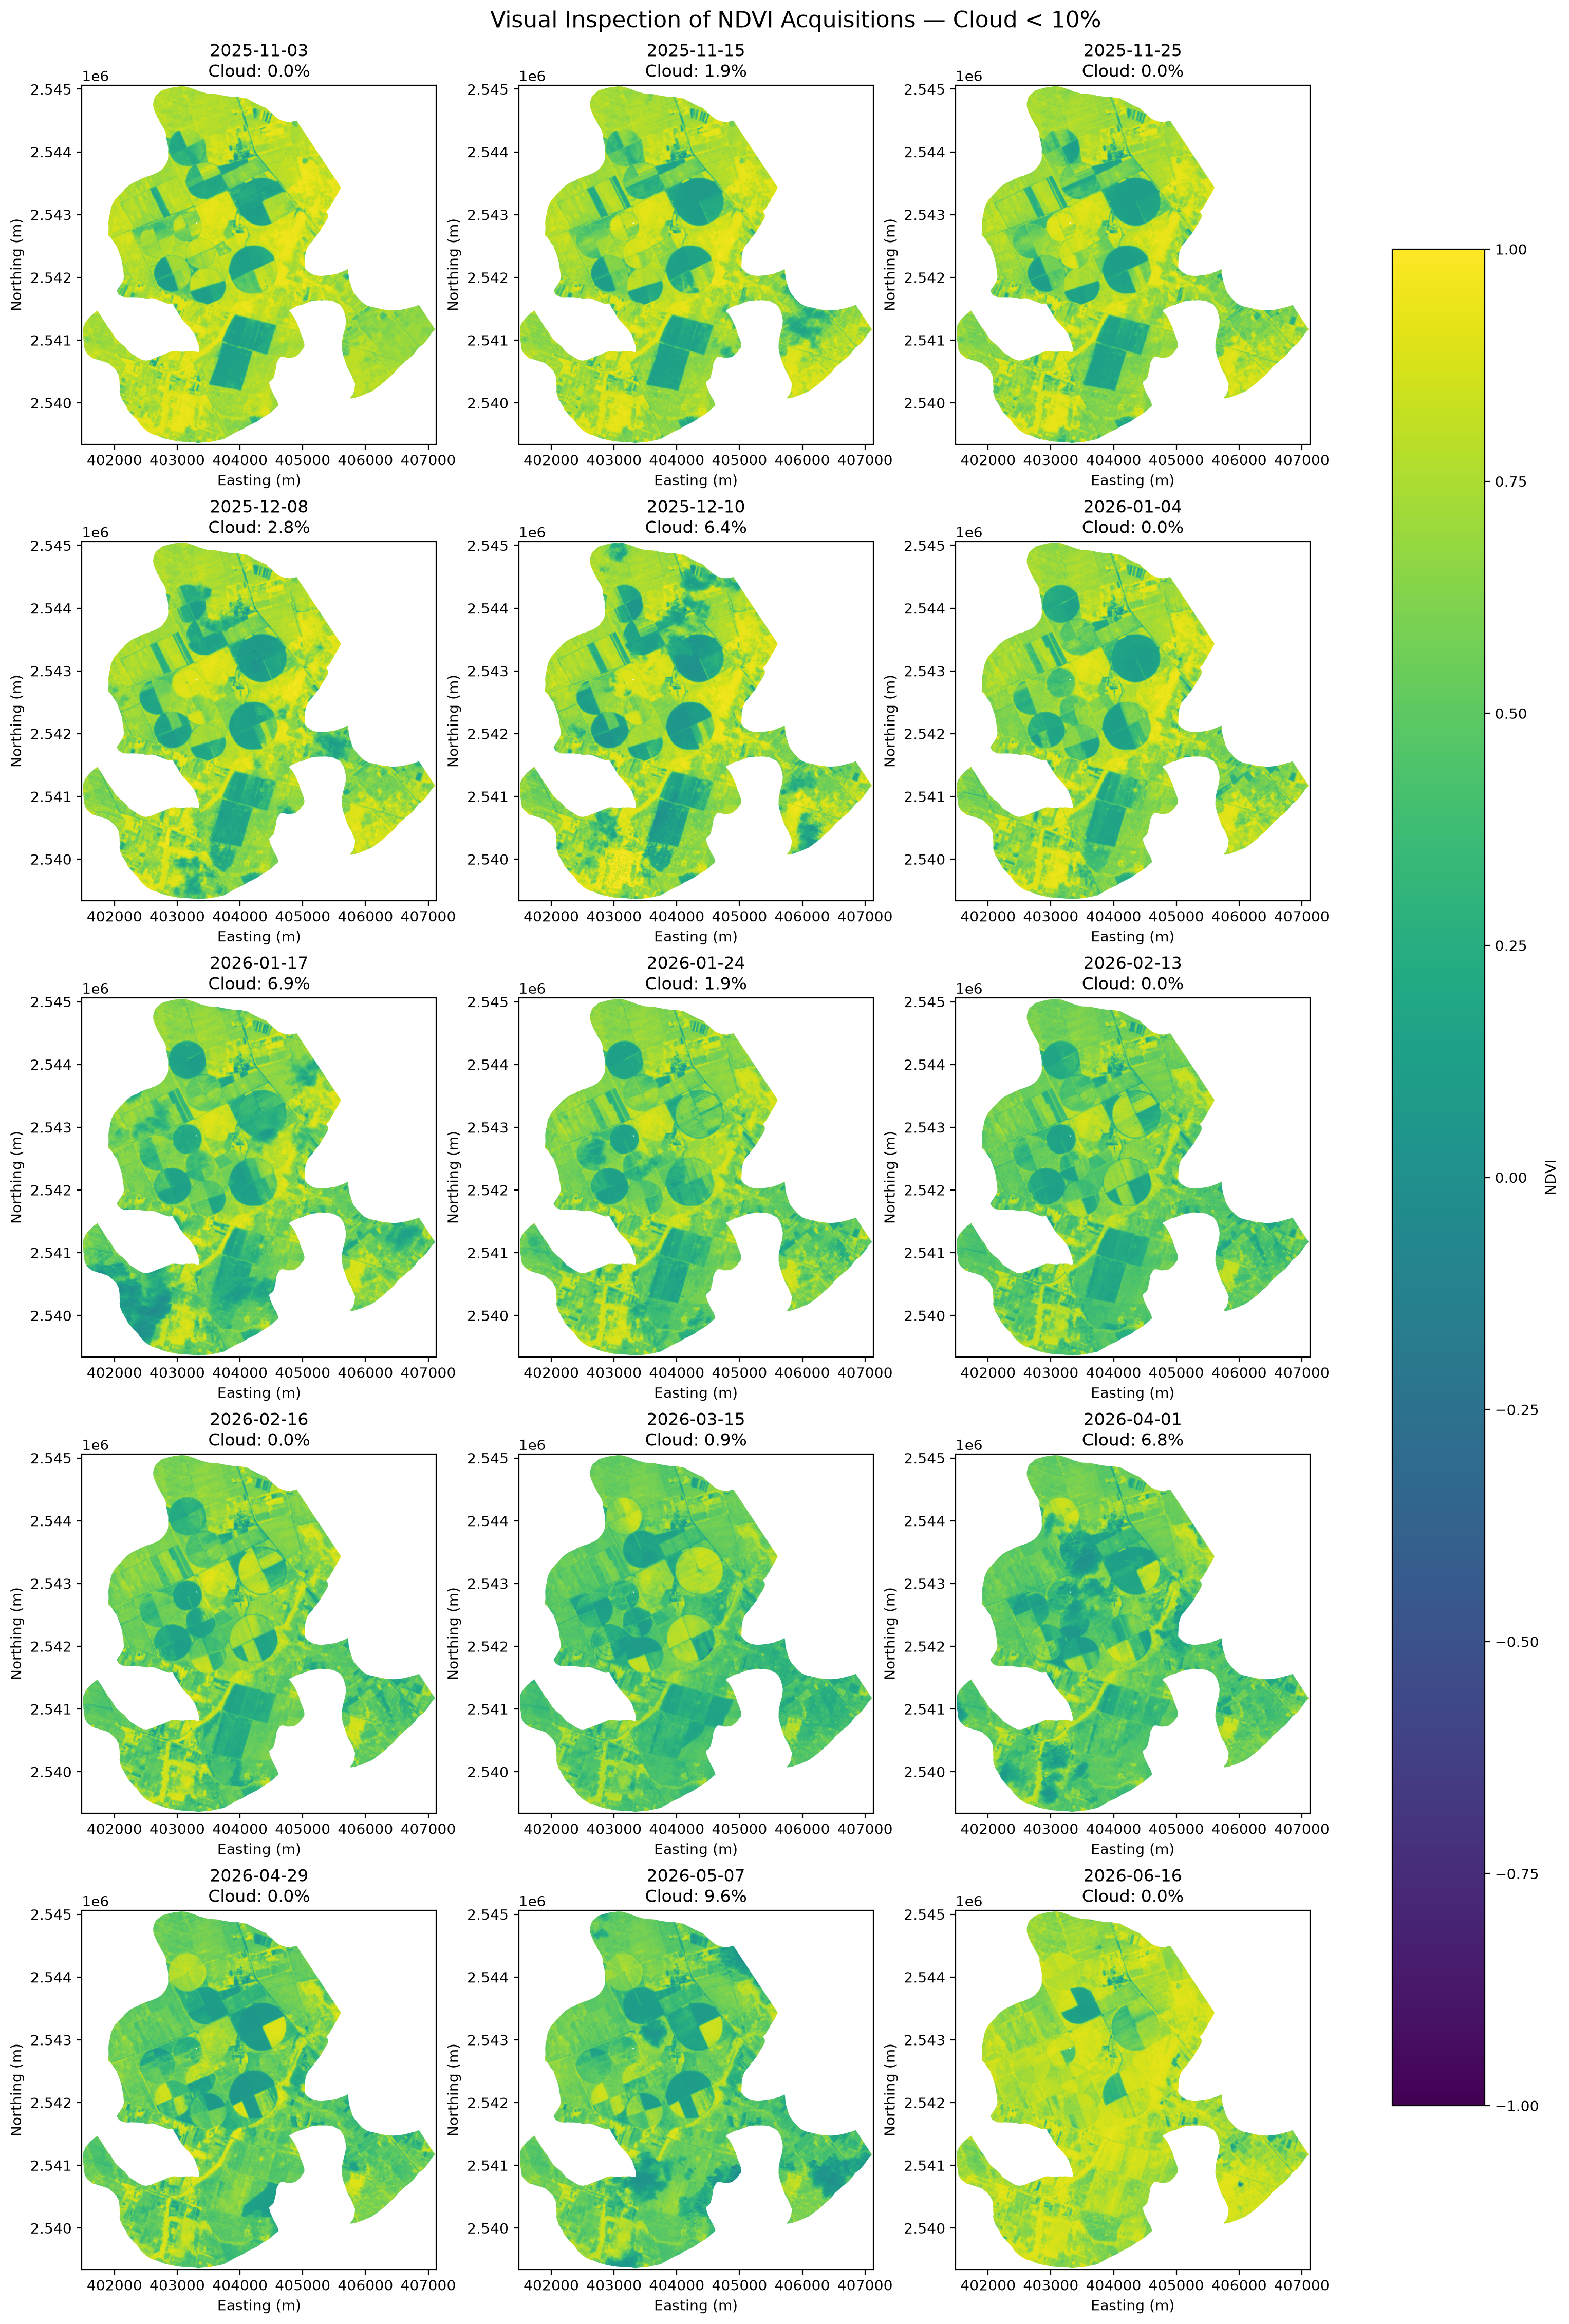
\includegraphics[
			width=\linewidth,
			height=5.3cm,
			keepaspectratio
			]{stage5_figure_59.png}
			
			\imagecaption{
				Cloud screening and observation selection.
			}
			
			\column{0.37\textwidth}
			
			\sectionlabel{Observation inventory}
			
			\metric{0.98\linewidth}{226}{Initial catalogue observations}
			
			\vspace{0.35cm}
			
			\metric{0.98\linewidth}{32}{Processed regional NDVI rasters}
			
			\vspace{0.35cm}
			
			\metric{0.98\linewidth}{15}{Retained regional acquisitions}
			
			\vspace{0.2cm}
			
			\pill{November 2025 -- June 2026}
			
			\vspace{0.2cm}
			
			{\scriptsize\color{muted}
				Regional screening threshold: cloud coverage below 10\%.
			}
			
		\end{columns}
		
	\end{frame}
	
	% ------------------------------------------------------------
	% 11. Regional temporal results
	% ------------------------------------------------------------
	
	\begin{frame}{Regional NDVI changes through time}
		
		\begin{columns}[T,onlytextwidth]
			
			\column{0.68\textwidth}
			
			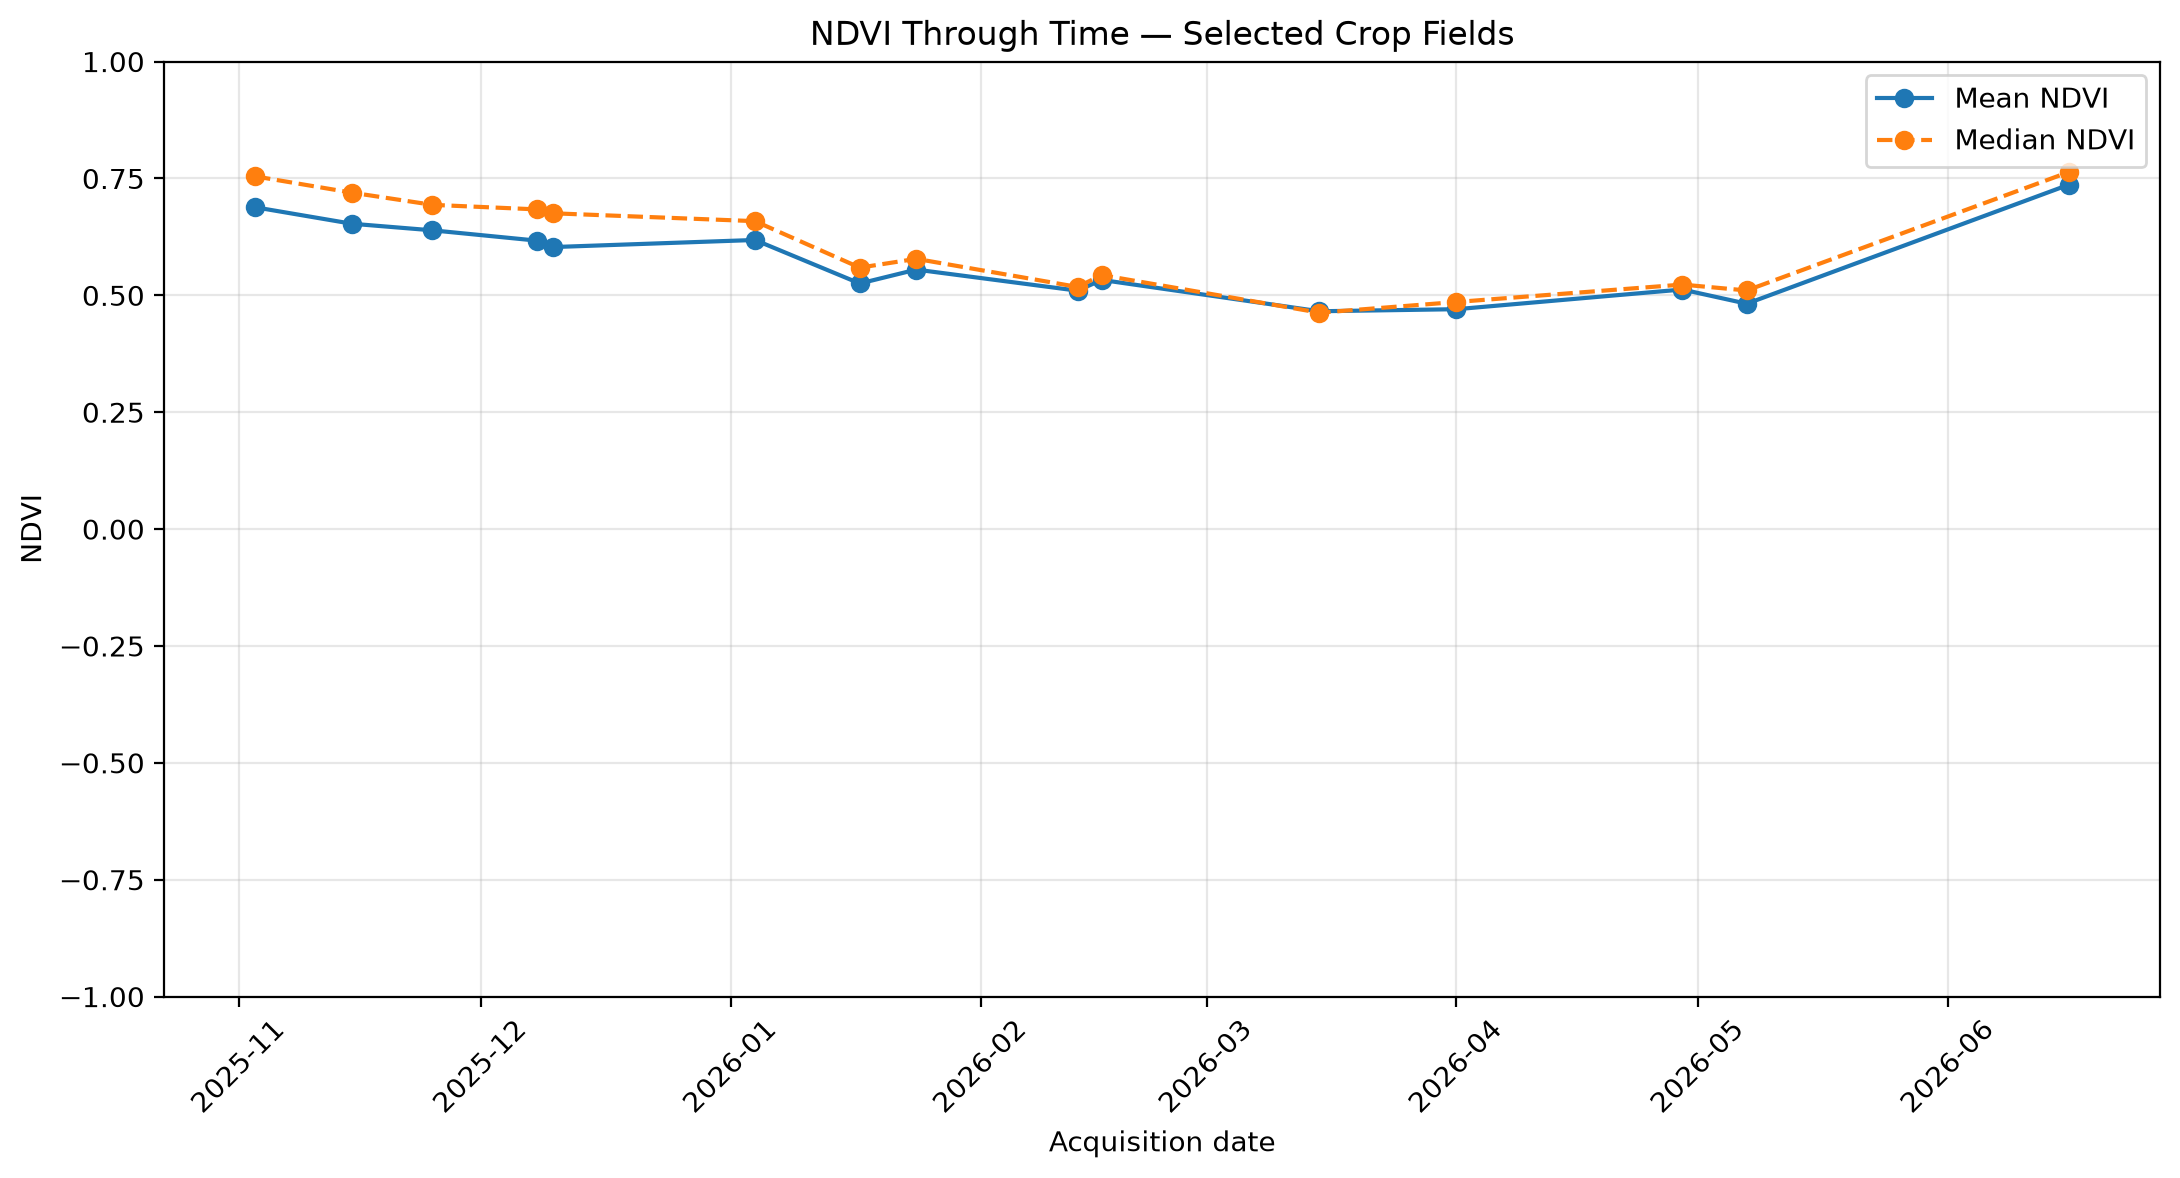
\includegraphics[
			width=\linewidth,
			height=5.3cm,
			keepaspectratio
			]{stage5_figure_67.png}
			
			\imagecaption{
				Mean and median NDVI across the selected agricultural region.
			}
			
			\column{0.28\textwidth}
			
			\sectionlabel{Mean NDVI}
			
			\metric{0.98\linewidth}{0.688}{3 November 2025}
			
			\vspace{0.35cm}
			
			\metric{0.98\linewidth}{0.466}{15 March 2026}
			
			\vspace{0.35cm}
			
			\metric{0.98\linewidth}{0.737}{16 June 2026}
			
		\end{columns}
		
		\vspace{0.15cm}
		
		\takeaway{
			Regional NDVI declined from November through March,
			then fluctuated and increased by June.
		}
		
	\end{frame}
	
	% ------------------------------------------------------------
	% 12. Spatial and distributional variation
	% ------------------------------------------------------------
	
	\begin{frame}{One average cannot describe every pixel}
		
		\begin{columns}[T,onlytextwidth]
			
			\column{0.50\textwidth}
			
			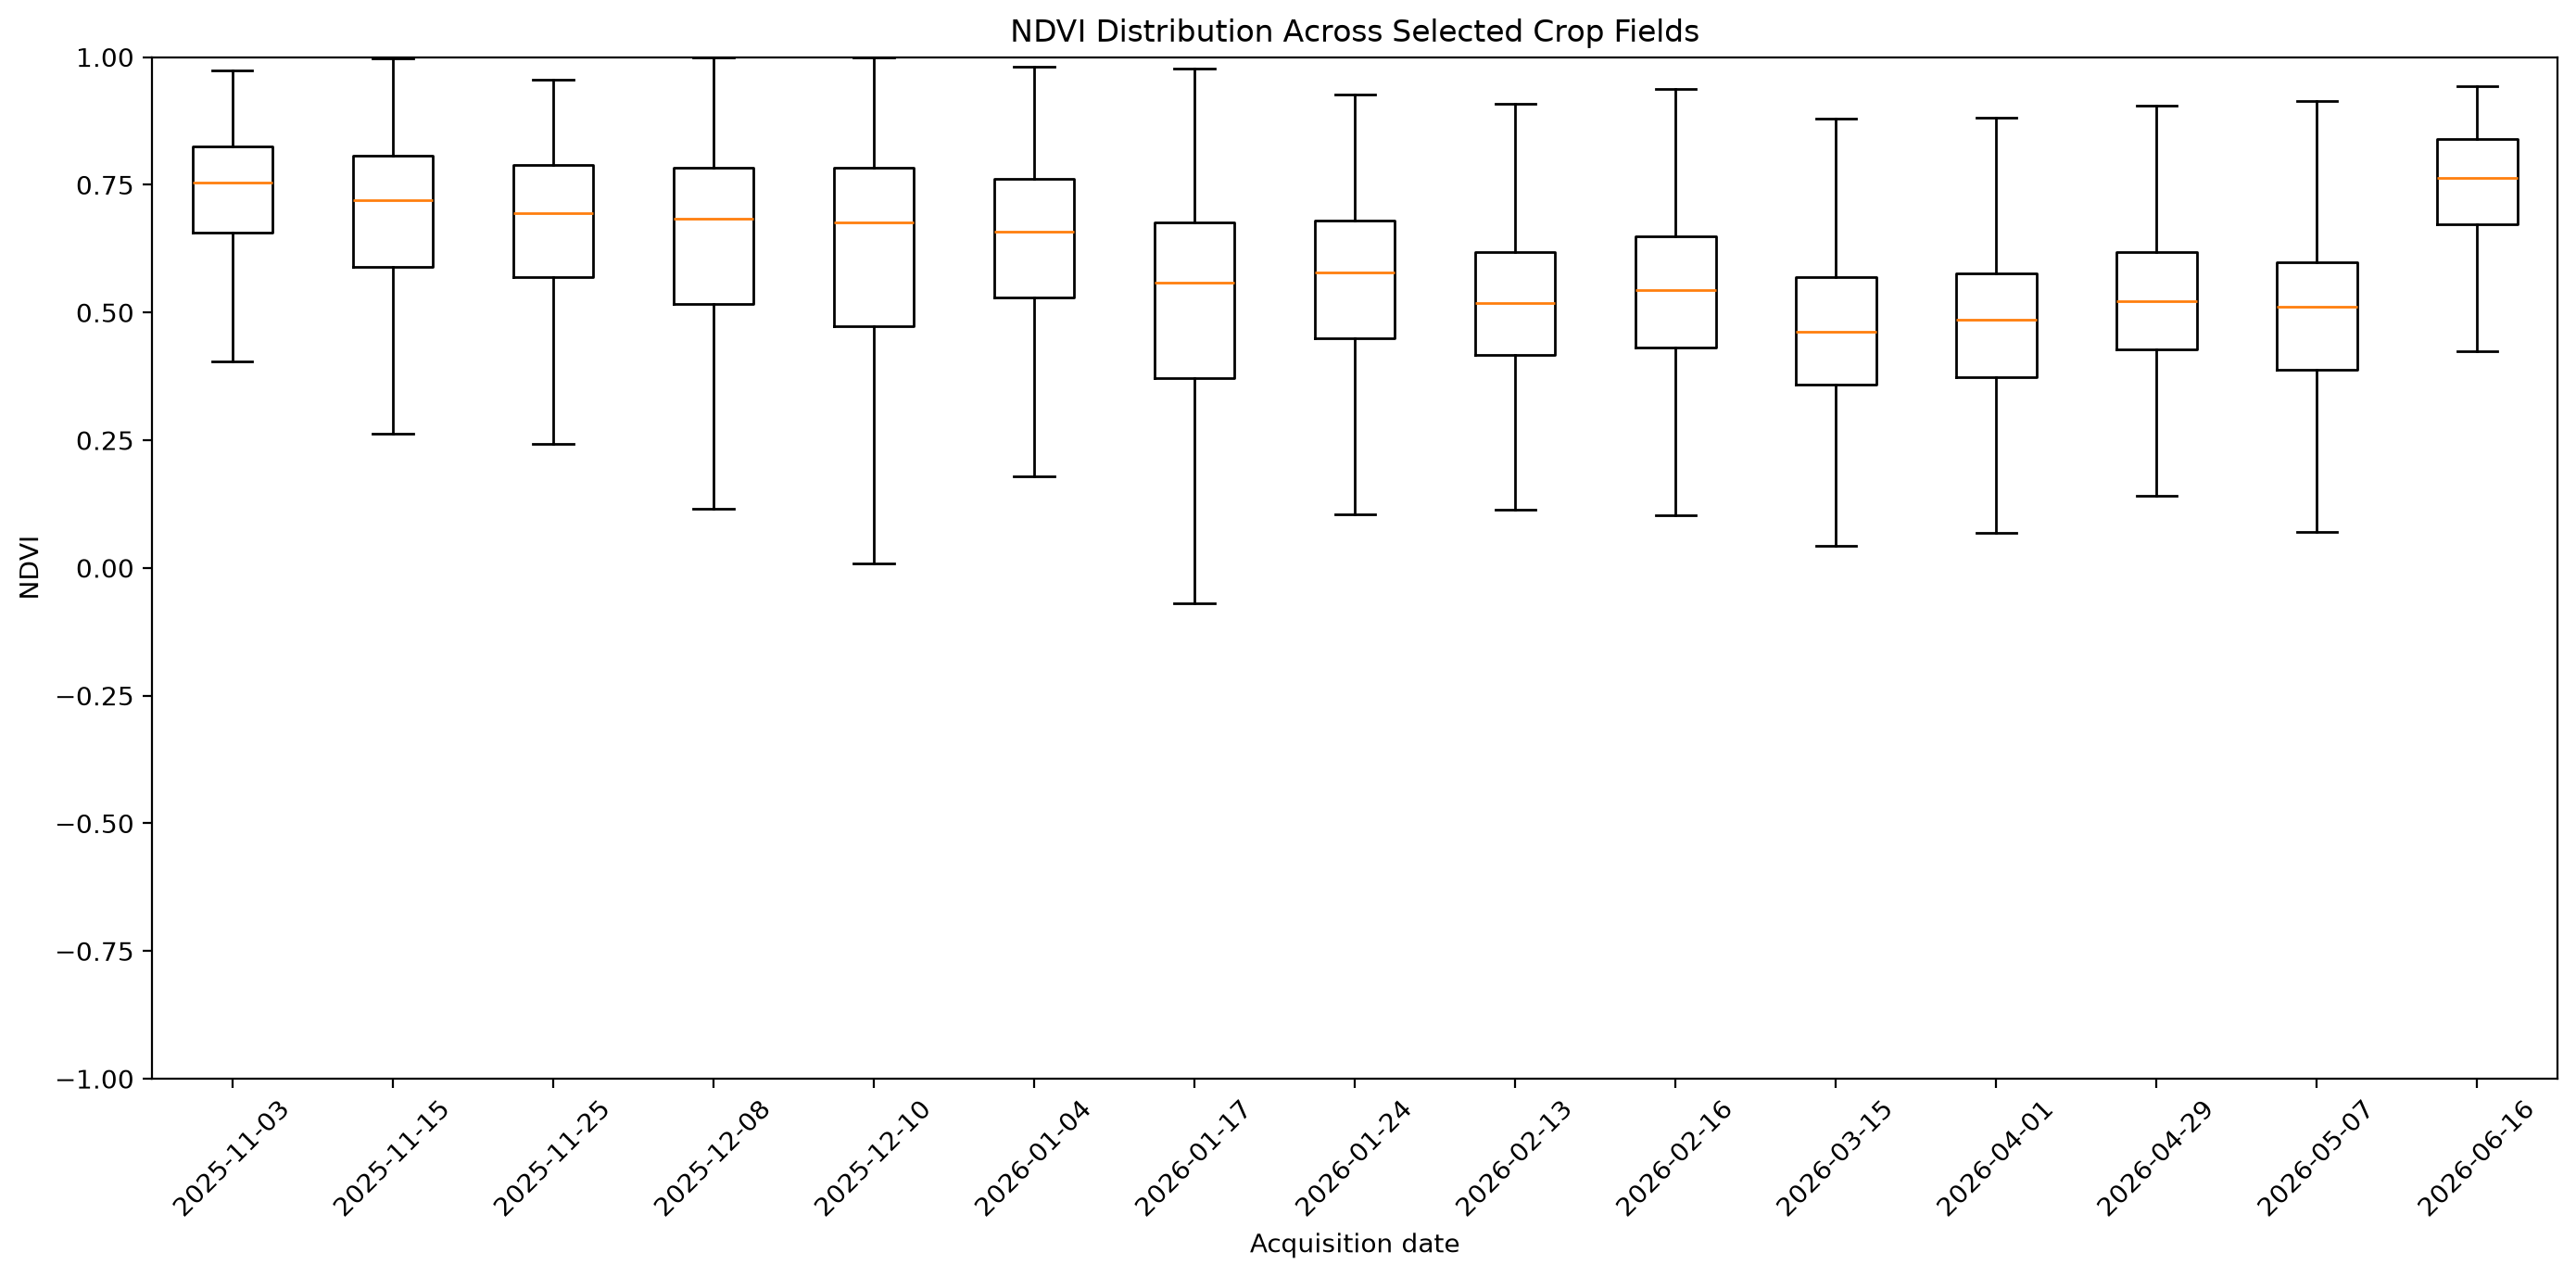
\includegraphics[
			width=\linewidth,
			height=4.8cm,
			keepaspectratio
			]{stage5_figure_70.png}
			
			\imagecaption{
				Regional NDVI distributions across acquisition dates.
			}
			
			\column{0.46\textwidth}
			
			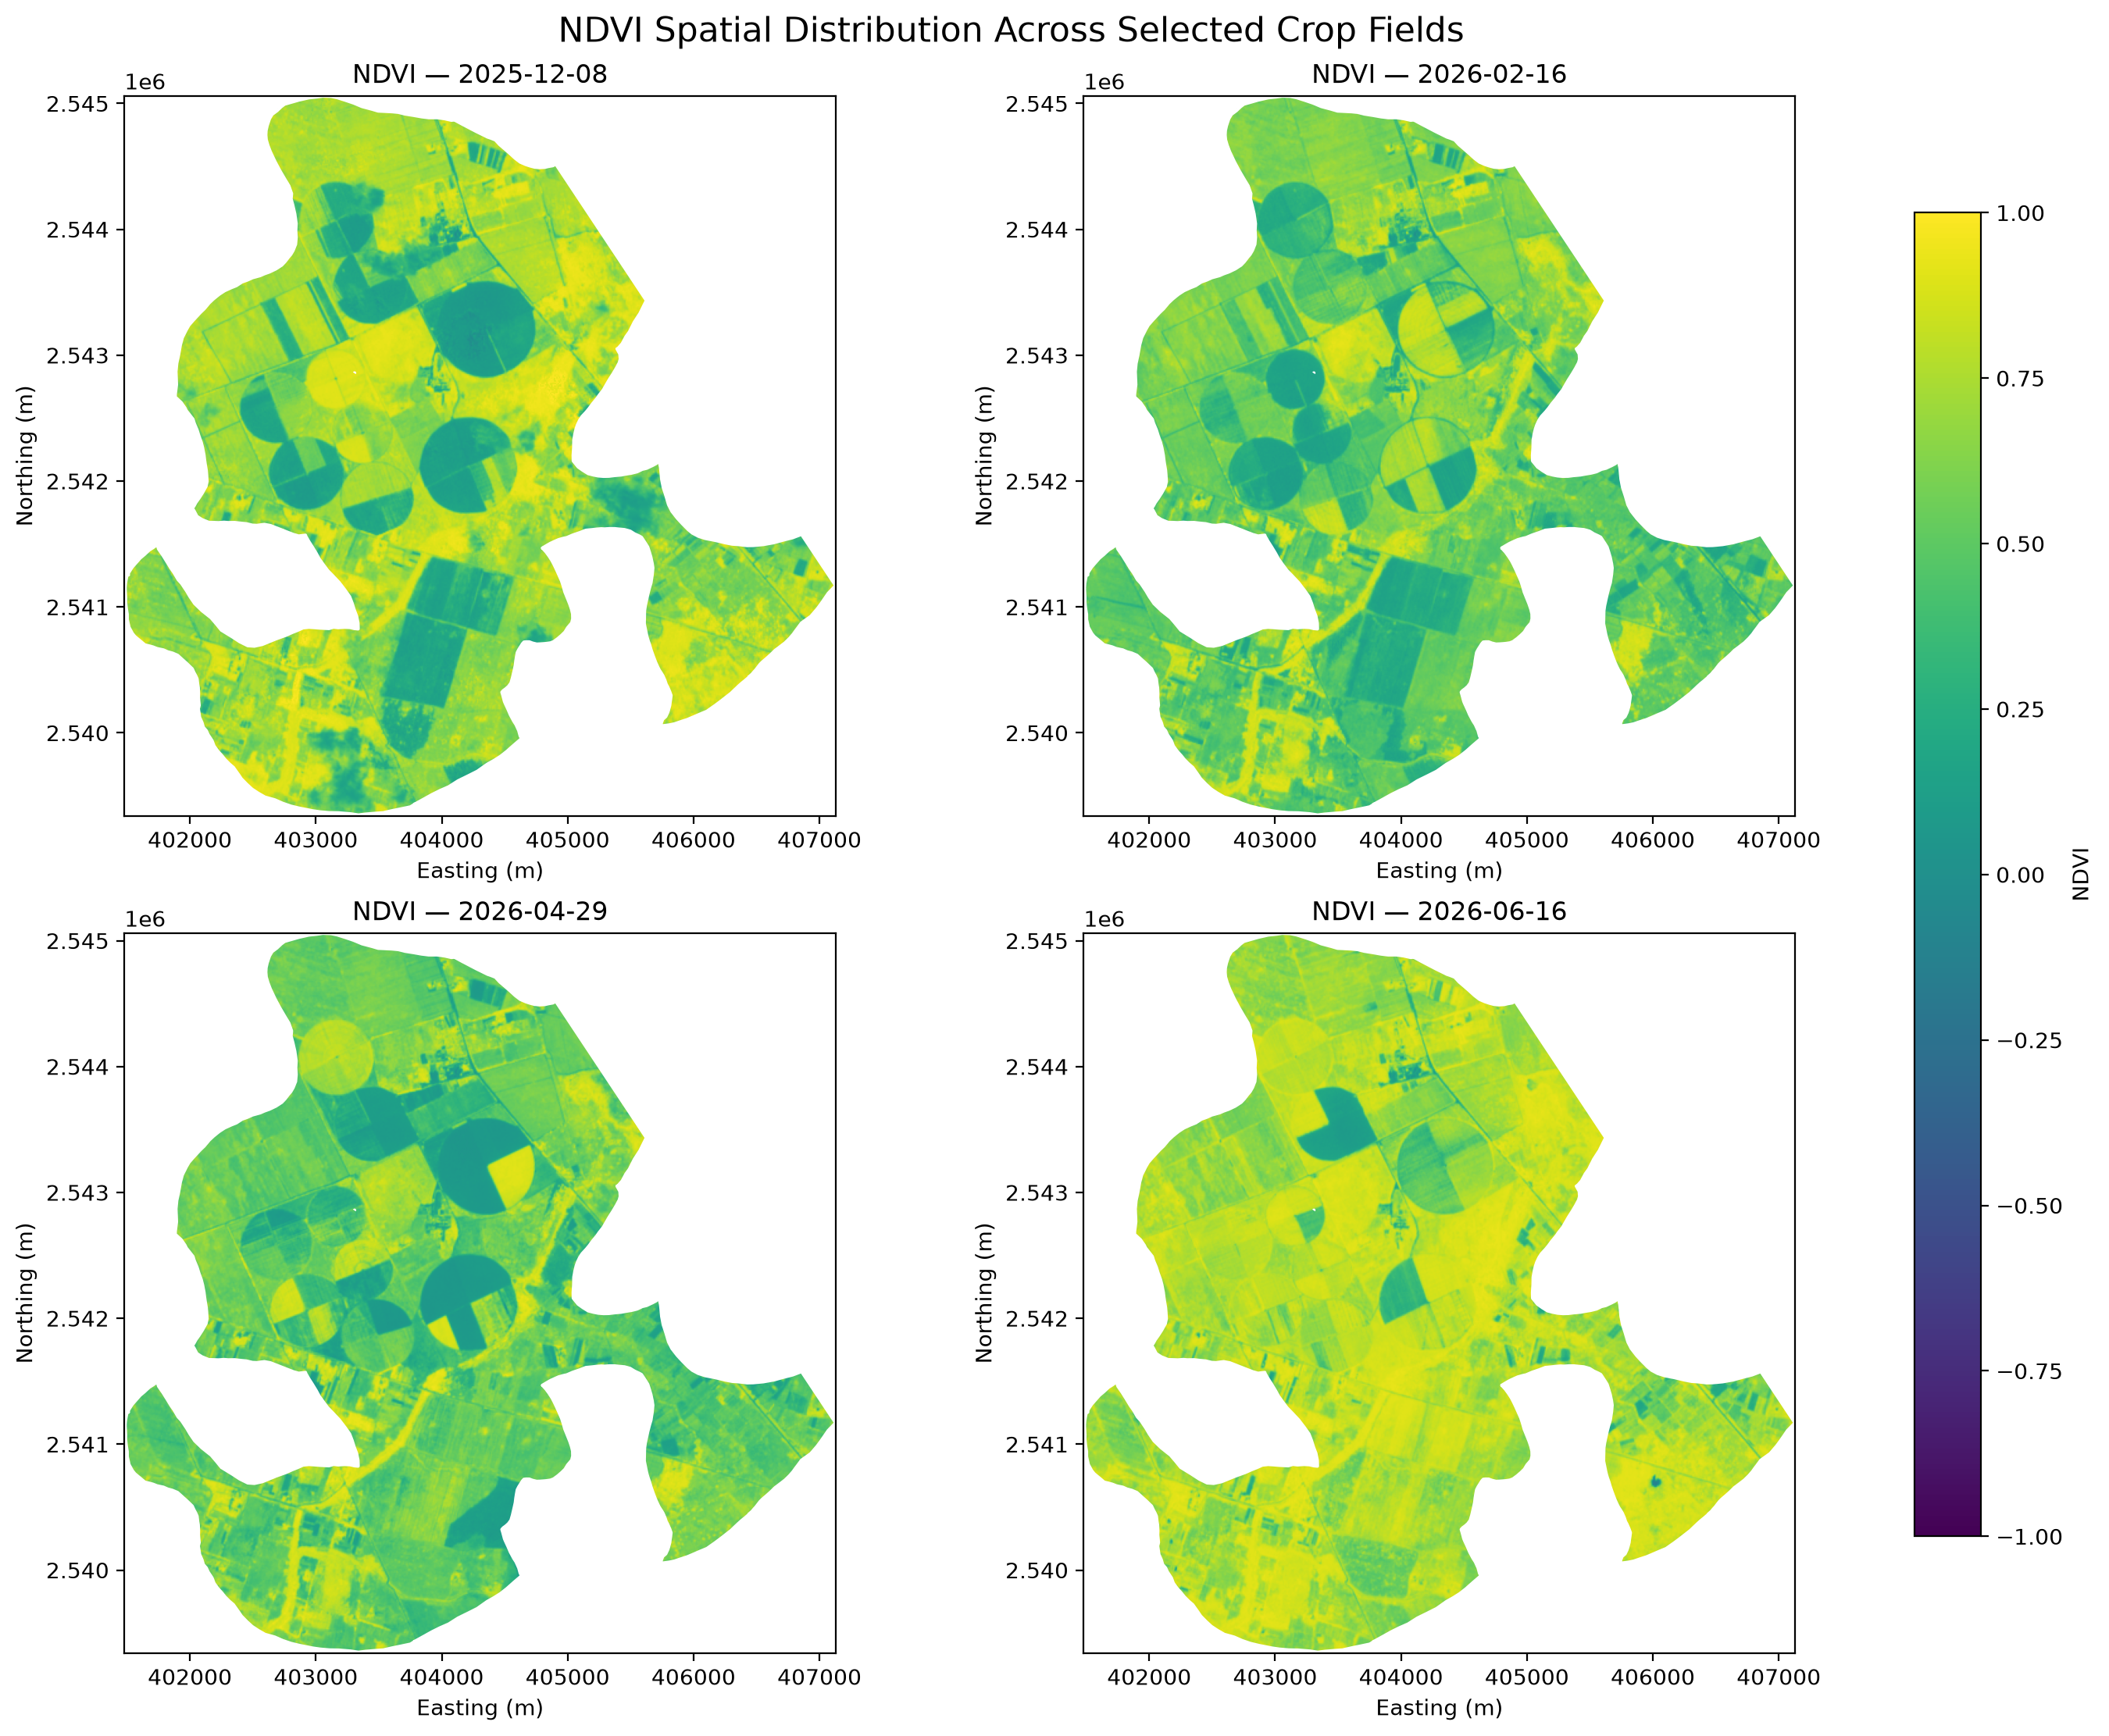
\includegraphics[
			width=\linewidth,
			height=4.8cm,
			keepaspectratio
			]{stage5_figure_76.png}
			
			\imagecaption{
				Spatial variation in NDVI across selected dates.
			}
			
		\end{columns}
		
		\vspace{0.2cm}
		
		\begin{beamercolorbox}[
			rounded=true,
			sep=0.18cm,
			wd=\linewidth
			]{block body}
			
			\small
			Distribution plots describe variation within the region;
			spatial maps show where vegetation-index values differ.
			Neither alone identifies the cause of those differences.
			
		\end{beamercolorbox}
		
	\end{frame}
	
	% ------------------------------------------------------------
	% 13. Selected agricultural region
	% ------------------------------------------------------------
	
	\begin{frame}{From the regional landscape to selected fields}
		
		\begin{columns}[T,onlytextwidth]
			
			\column{0.59\textwidth}
			
			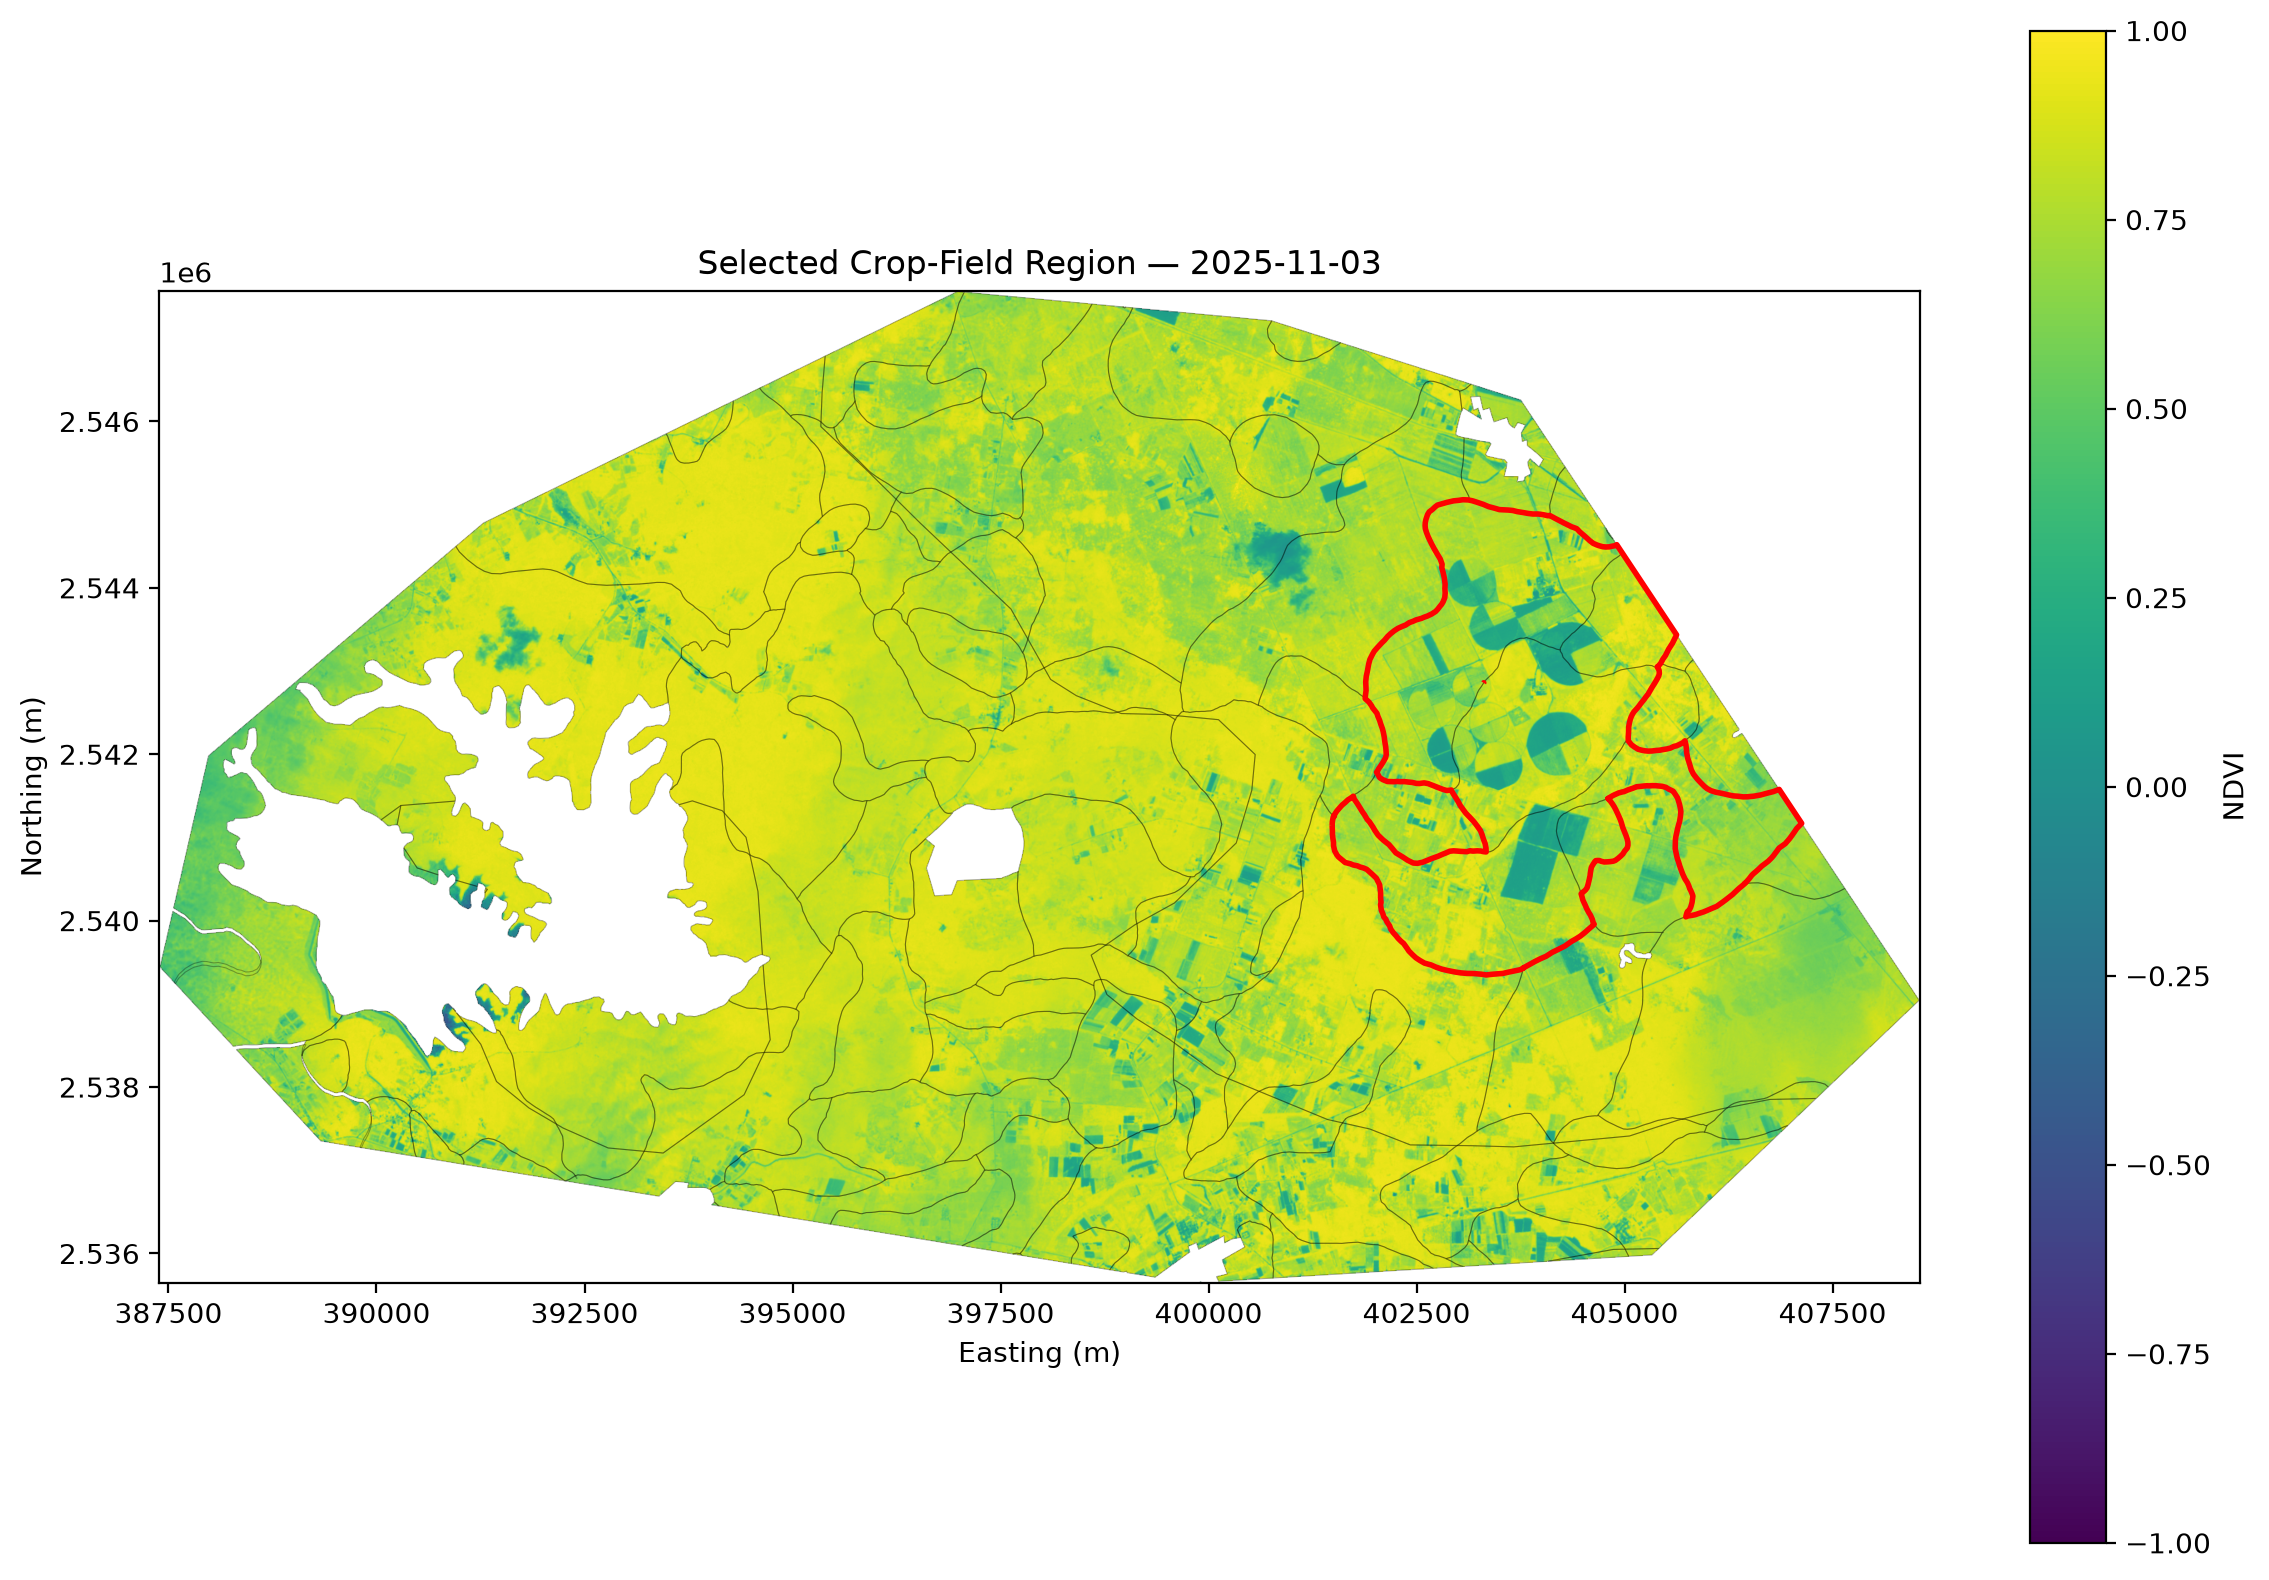
\includegraphics[
			width=\linewidth,
			height=5.4cm,
			keepaspectratio
			]{stage5_figure_41.png}
			
			\imagecaption{
				Selected agricultural region used for NDVI analysis.
			}
			
			\column{0.37\textwidth}
			
			\sectionlabel{Field-level comparison}
			
			{\large\bfseries
				Three locally verified potato fields
			}
			
			\vspace{0.25cm}
			
			\begin{itemize}
				\item Sampling polygons digitized in QGIS.
				\item NDVI extracted across 15 accepted dates.
				\item Field-specific temporal patterns compared.
				\item Regional averages interpreted alongside local variation.
			\end{itemize}
			
			\vspace{0.2cm}
			
			\metric{0.98\linewidth}{45}{Field-date observations}
			
		\end{columns}
		
	\end{frame}
	
	% ------------------------------------------------------------
	% 14. Field samples
	% ------------------------------------------------------------
	
	\begin{frame}{Three selected potato-field samples}
		
		\begin{columns}[T,onlytextwidth]
			
			\column{0.65\textwidth}
			
			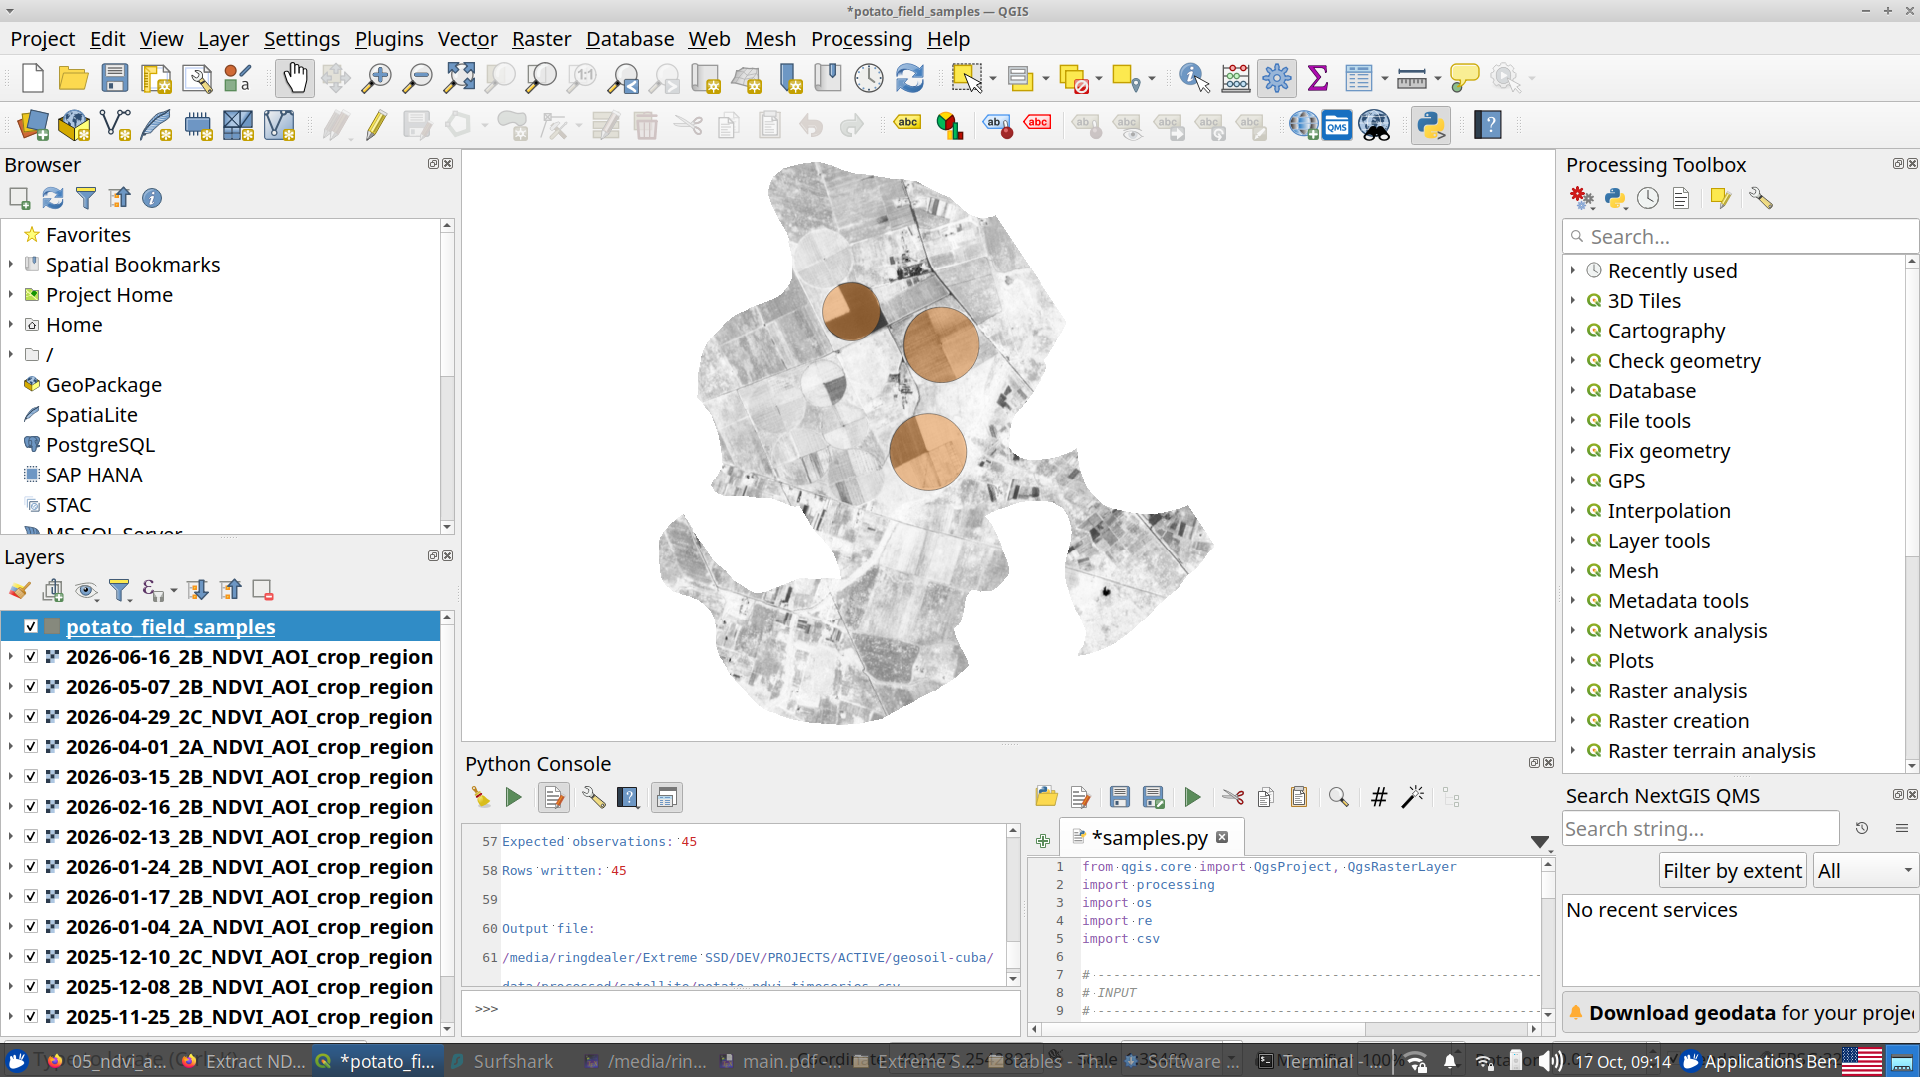
\includegraphics[
			width=\linewidth,
			height=5.6cm,
			keepaspectratio
			]{potato_samples.png}
			
			\imagecaption{
				Three sampling polygons displayed over the agricultural-region NDVI raster.
			}
			
			\column{0.31\textwidth}
			
			\sectionlabel{Sampling design}
			
			\metric{0.98\linewidth}{3}{Selected fields}
			
			\vspace{0.35cm}
			
			\metric{0.98\linewidth}{15}{Acquisition dates}
			
			\vspace{0.35cm}
			
			\metric{0.98\linewidth}{45}{Field-date observations}
			
			\vspace{0.35cm}
			
			{\scriptsize\color{muted}
				Targeted samples, not a statistically representative
				survey of potato cultivation in Cuba.
			}
			
		\end{columns}
		
	\end{frame}
	
	% ------------------------------------------------------------
	% 15. Field-level temporal results
	% ------------------------------------------------------------
	
	\begin{frame}{Different fields, different NDVI trajectories}
		
		\begin{columns}[T,onlytextwidth]
			
			\column{0.69\textwidth}
			
			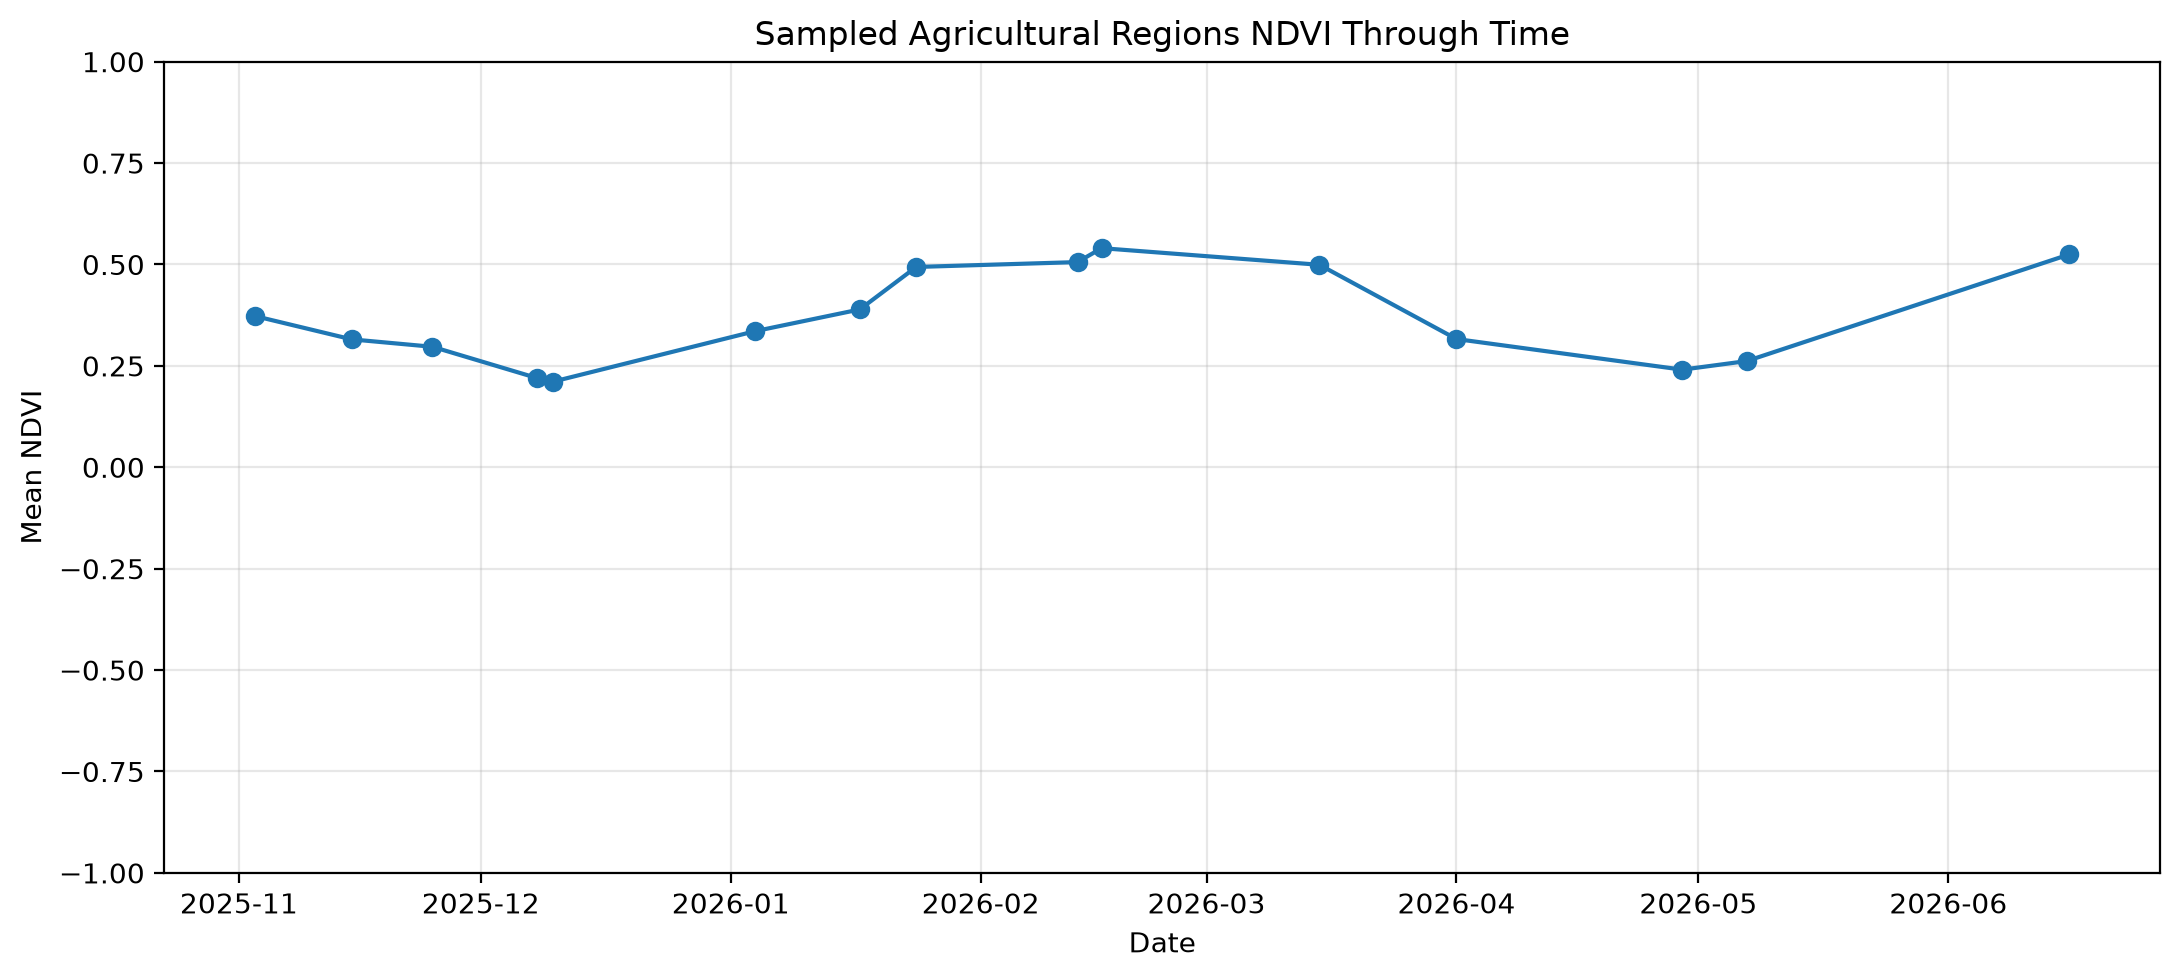
\includegraphics[
			width=\linewidth,
			height=5.2cm,
			keepaspectratio
			]{stage5_figure_84.png}
			
			\imagecaption{
				Mean NDVI through time for the three selected fields.
			}
			
			\column{0.27\textwidth}
			
			\sectionlabel{Observed maxima}
			
			{\small\bfseries Field 1}
			
			{\color{forest}\Large 0.744}
			
			{\scriptsize 15 March 2026}
			
			\vspace{0.35cm}
			
			{\small\bfseries Field 2}
			
			{\color{forest}\Large 0.690}
			
			{\scriptsize 16 June 2026}
			
			\vspace{0.35cm}
			
			{\small\bfseries Field 3}
			
			{\color{forest}\Large 0.573}
			
			{\scriptsize 24 January 2026}
			
		\end{columns}
		
		\takeaway{
			The sampled fields reached their highest observed mean
			NDVI values on different dates.
		}
		
	\end{frame}
	
	% ------------------------------------------------------------
	% 16. Limitations
	% ------------------------------------------------------------
	
	\begin{frame}{What the results can -- and cannot -- tell us}
		
		\begin{columns}[T,onlytextwidth]
			
			\column{0.48\textwidth}
			
			\begin{beamercolorbox}[
				rounded=true,
				sep=0.25cm,
				wd=\linewidth
				]{block body}
				
				{\large\bfseries\color{forest}
					Supported by this workflow}
				
				\vspace{0.2cm}
				
				\begin{itemize}
					\item Reported soil-map coverage and gaps.
					\item Detected polygon overlaps.
					\item Temporal variation in NDVI.
					\item Differences between selected field samples.
				\end{itemize}
				
			\end{beamercolorbox}
			
			\column{0.48\textwidth}
			
			\begin{beamercolorbox}[
				rounded=true,
				sep=0.25cm,
				wd=\linewidth
				]{block body}
				
				{\large\bfseries\color{forest}
					Not established by NDVI alone}
				
				\vspace{0.2cm}
				
				\begin{itemize}
					\item Crop yield or productivity.
					\item Exact crop phenological stages.
					\item Causal effects of soil classes on NDVI.
					\item Representative conditions across Cuba.
				\end{itemize}
				
			\end{beamercolorbox}
			
		\end{columns}
		
		\vspace{0.35cm}
		
		\begin{center}
			\textcolor{forest}{
				\bfseries
				Data quality and uncertainty matter as much as visualization.
			}
		\end{center}
		
	\end{frame}
	
	% ------------------------------------------------------------
	% 17. Conclusions
	% ------------------------------------------------------------
	
	\begin{frame}{What GeoSoil-Cuba demonstrates}
		
		\begin{columns}[T,onlytextwidth]
			
			\column{0.31\textwidth}
			
			\begin{beamercolorbox}[
				rounded=true,
				sep=0.22cm,
				wd=\linewidth
				]{block body}
				
				{\color{leaf}\Large\bfseries 01}
				
				\vspace{0.15cm}
				
				{\large\bfseries
					Spatial data quality}
				
				\vspace{0.15cm}
				
				\small
				Coverage, geometry, and topology
				should be assessed before interpretation.
				
			\end{beamercolorbox}
			
			\column{0.31\textwidth}
			
			\begin{beamercolorbox}[
				rounded=true,
				sep=0.22cm,
				wd=\linewidth
				]{block body}
				
				{\color{leaf}\Large\bfseries 02}
				
				\vspace{0.15cm}
				
				{\large\bfseries
					Satellite analysis}
				
				\vspace{0.15cm}
				
				\small
				Sentinel-2 NDVI supports the
				analysis of vegetation-index dynamics.
				
			\end{beamercolorbox}
			
			\column{0.31\textwidth}
			
			\begin{beamercolorbox}[
				rounded=true,
				sep=0.22cm,
				wd=\linewidth
				]{block body}
				
				{\color{leaf}\Large\bfseries 03}
				
				\vspace{0.15cm}
				
				{\large\bfseries
					Reproducibility}
				
				\vspace{0.15cm}
				
				\small
				Open-source tools connect
				data preparation, analysis, and visualization.
				
			\end{beamercolorbox}
			
		\end{columns}
		
		\vspace{0.55cm}
		
		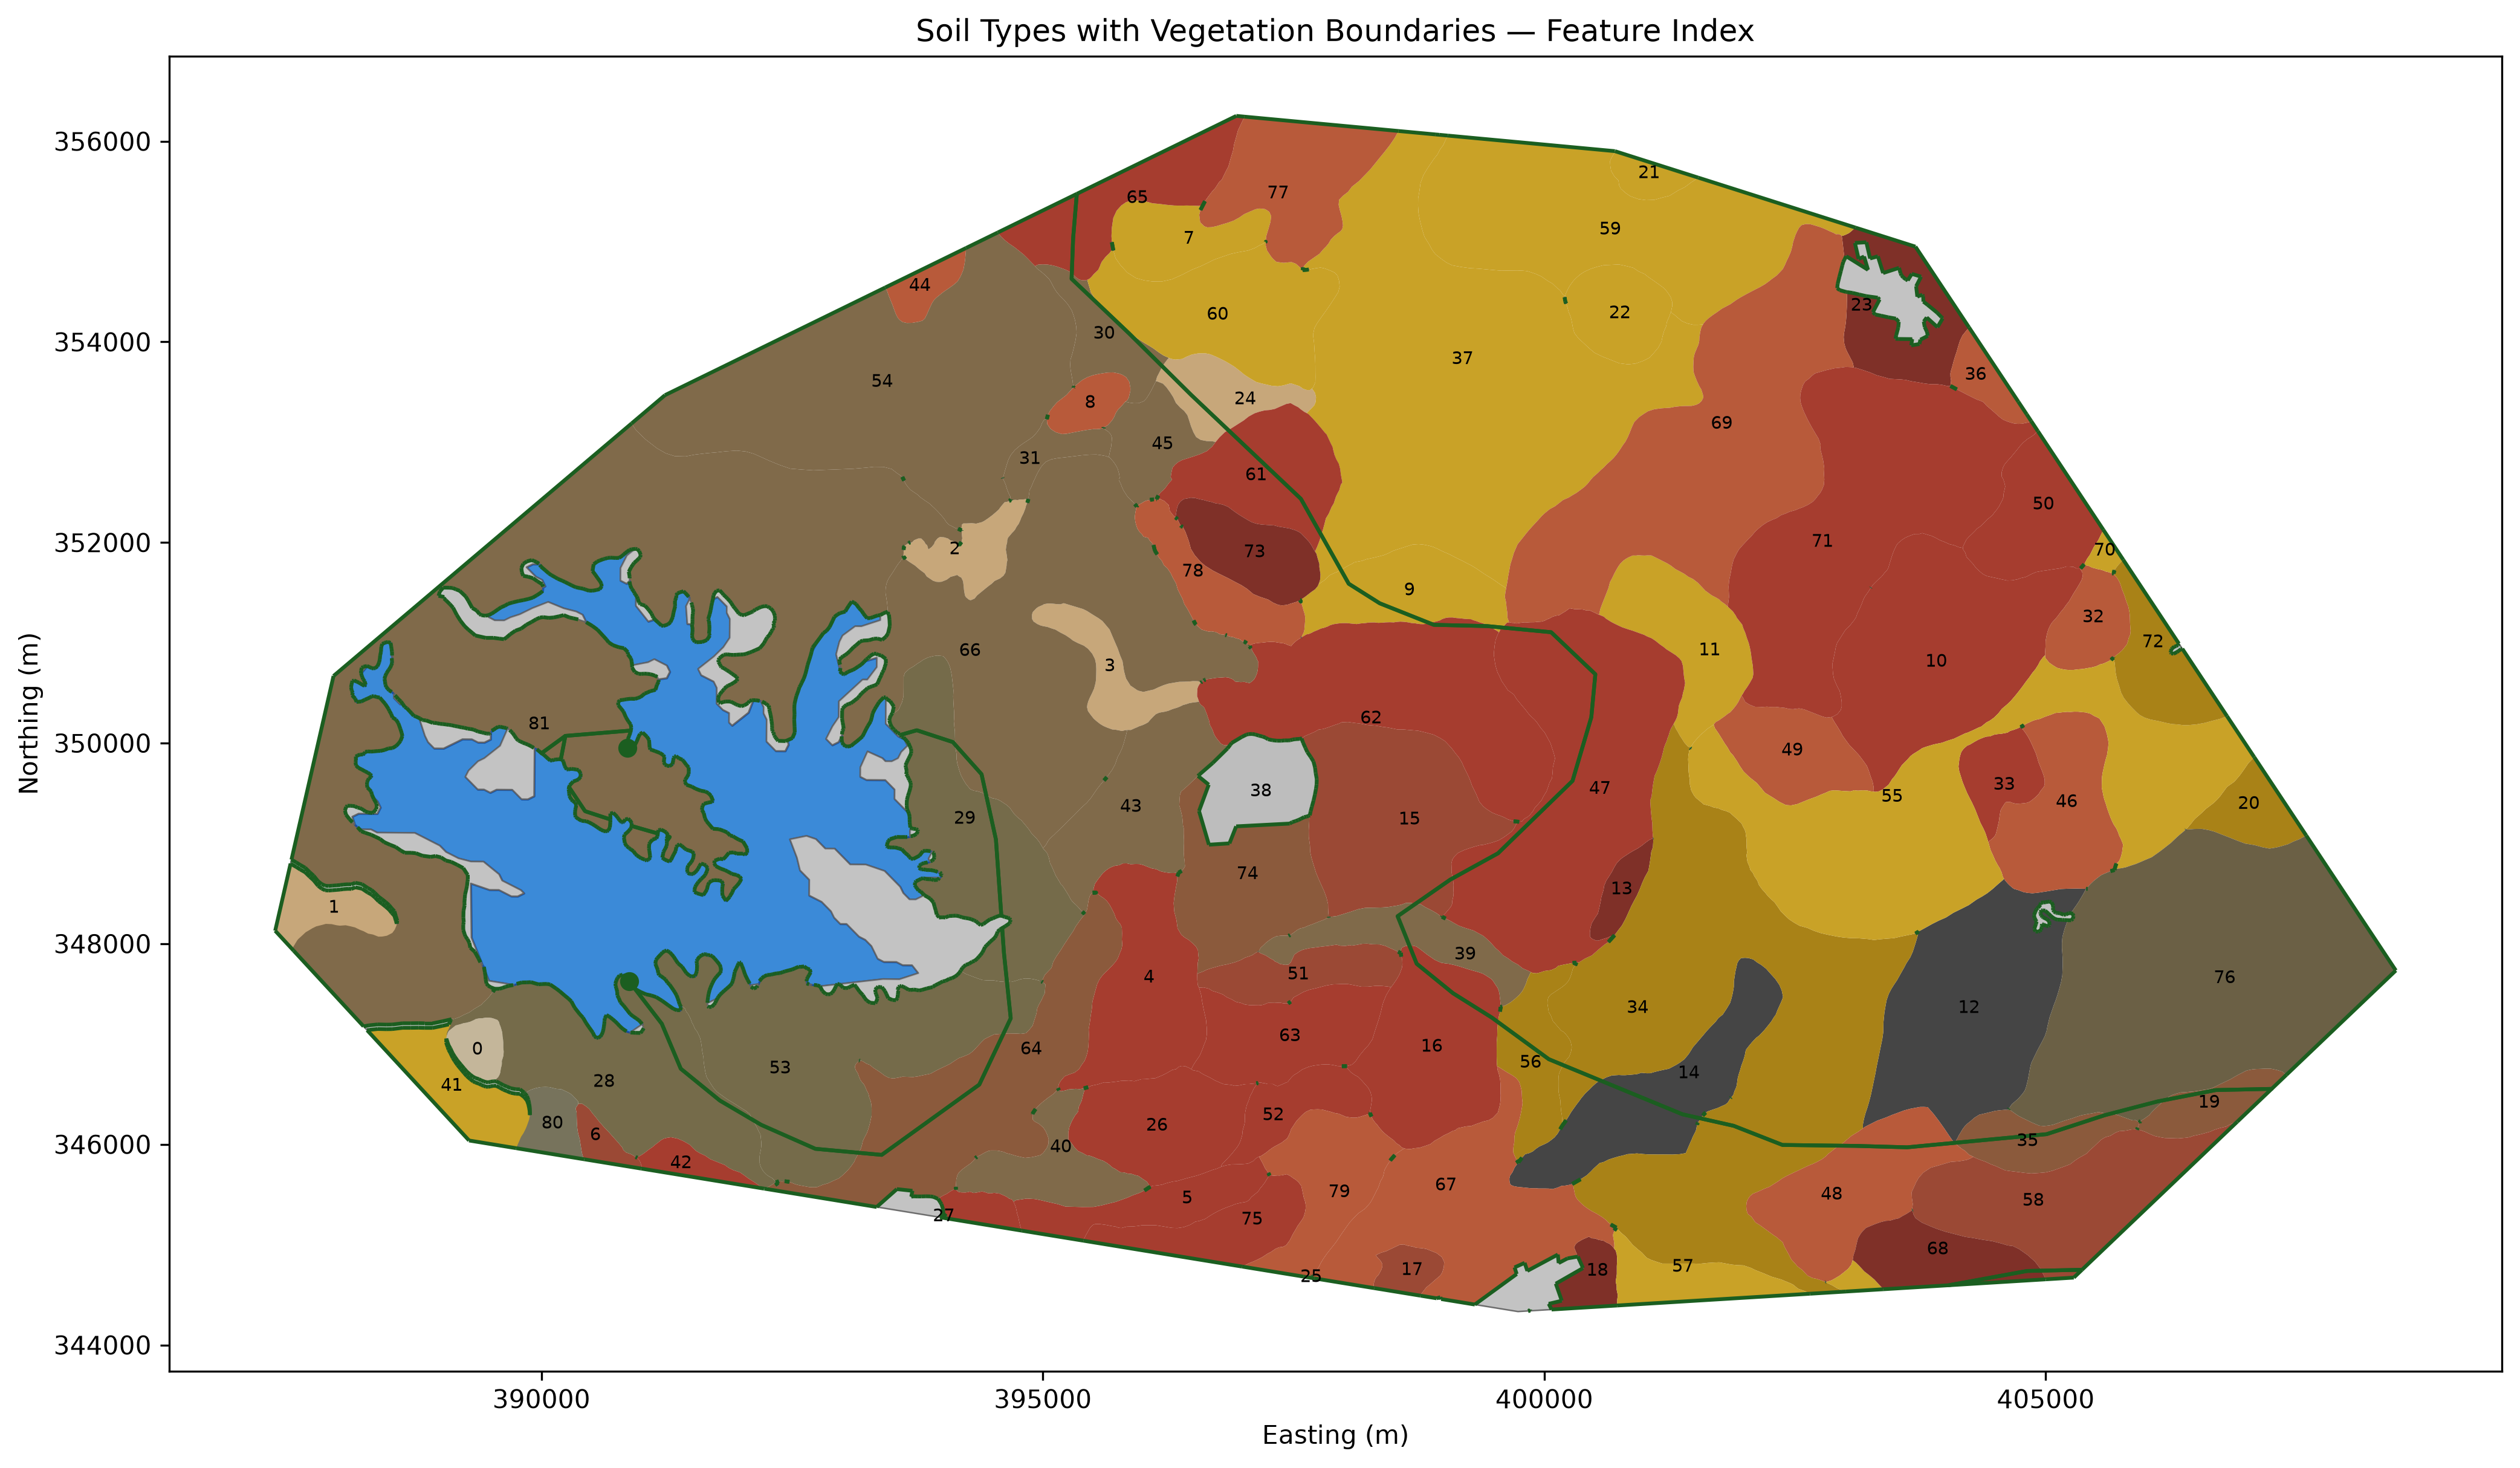
\includegraphics[
		width=\linewidth,
		height=2.3cm,
		keepaspectratio
		]{soil_types_with_vegetation_boundaries.png}
		
	\end{frame}
	
	% ------------------------------------------------------------
	% 18. Closing
	% ------------------------------------------------------------
	
	\begin{frame}[plain]
		
		\begin{tikzpicture}[remember picture,overlay]
			
			\node[
			anchor=south west,
			inner sep=0
			] at (current page.south west) {
				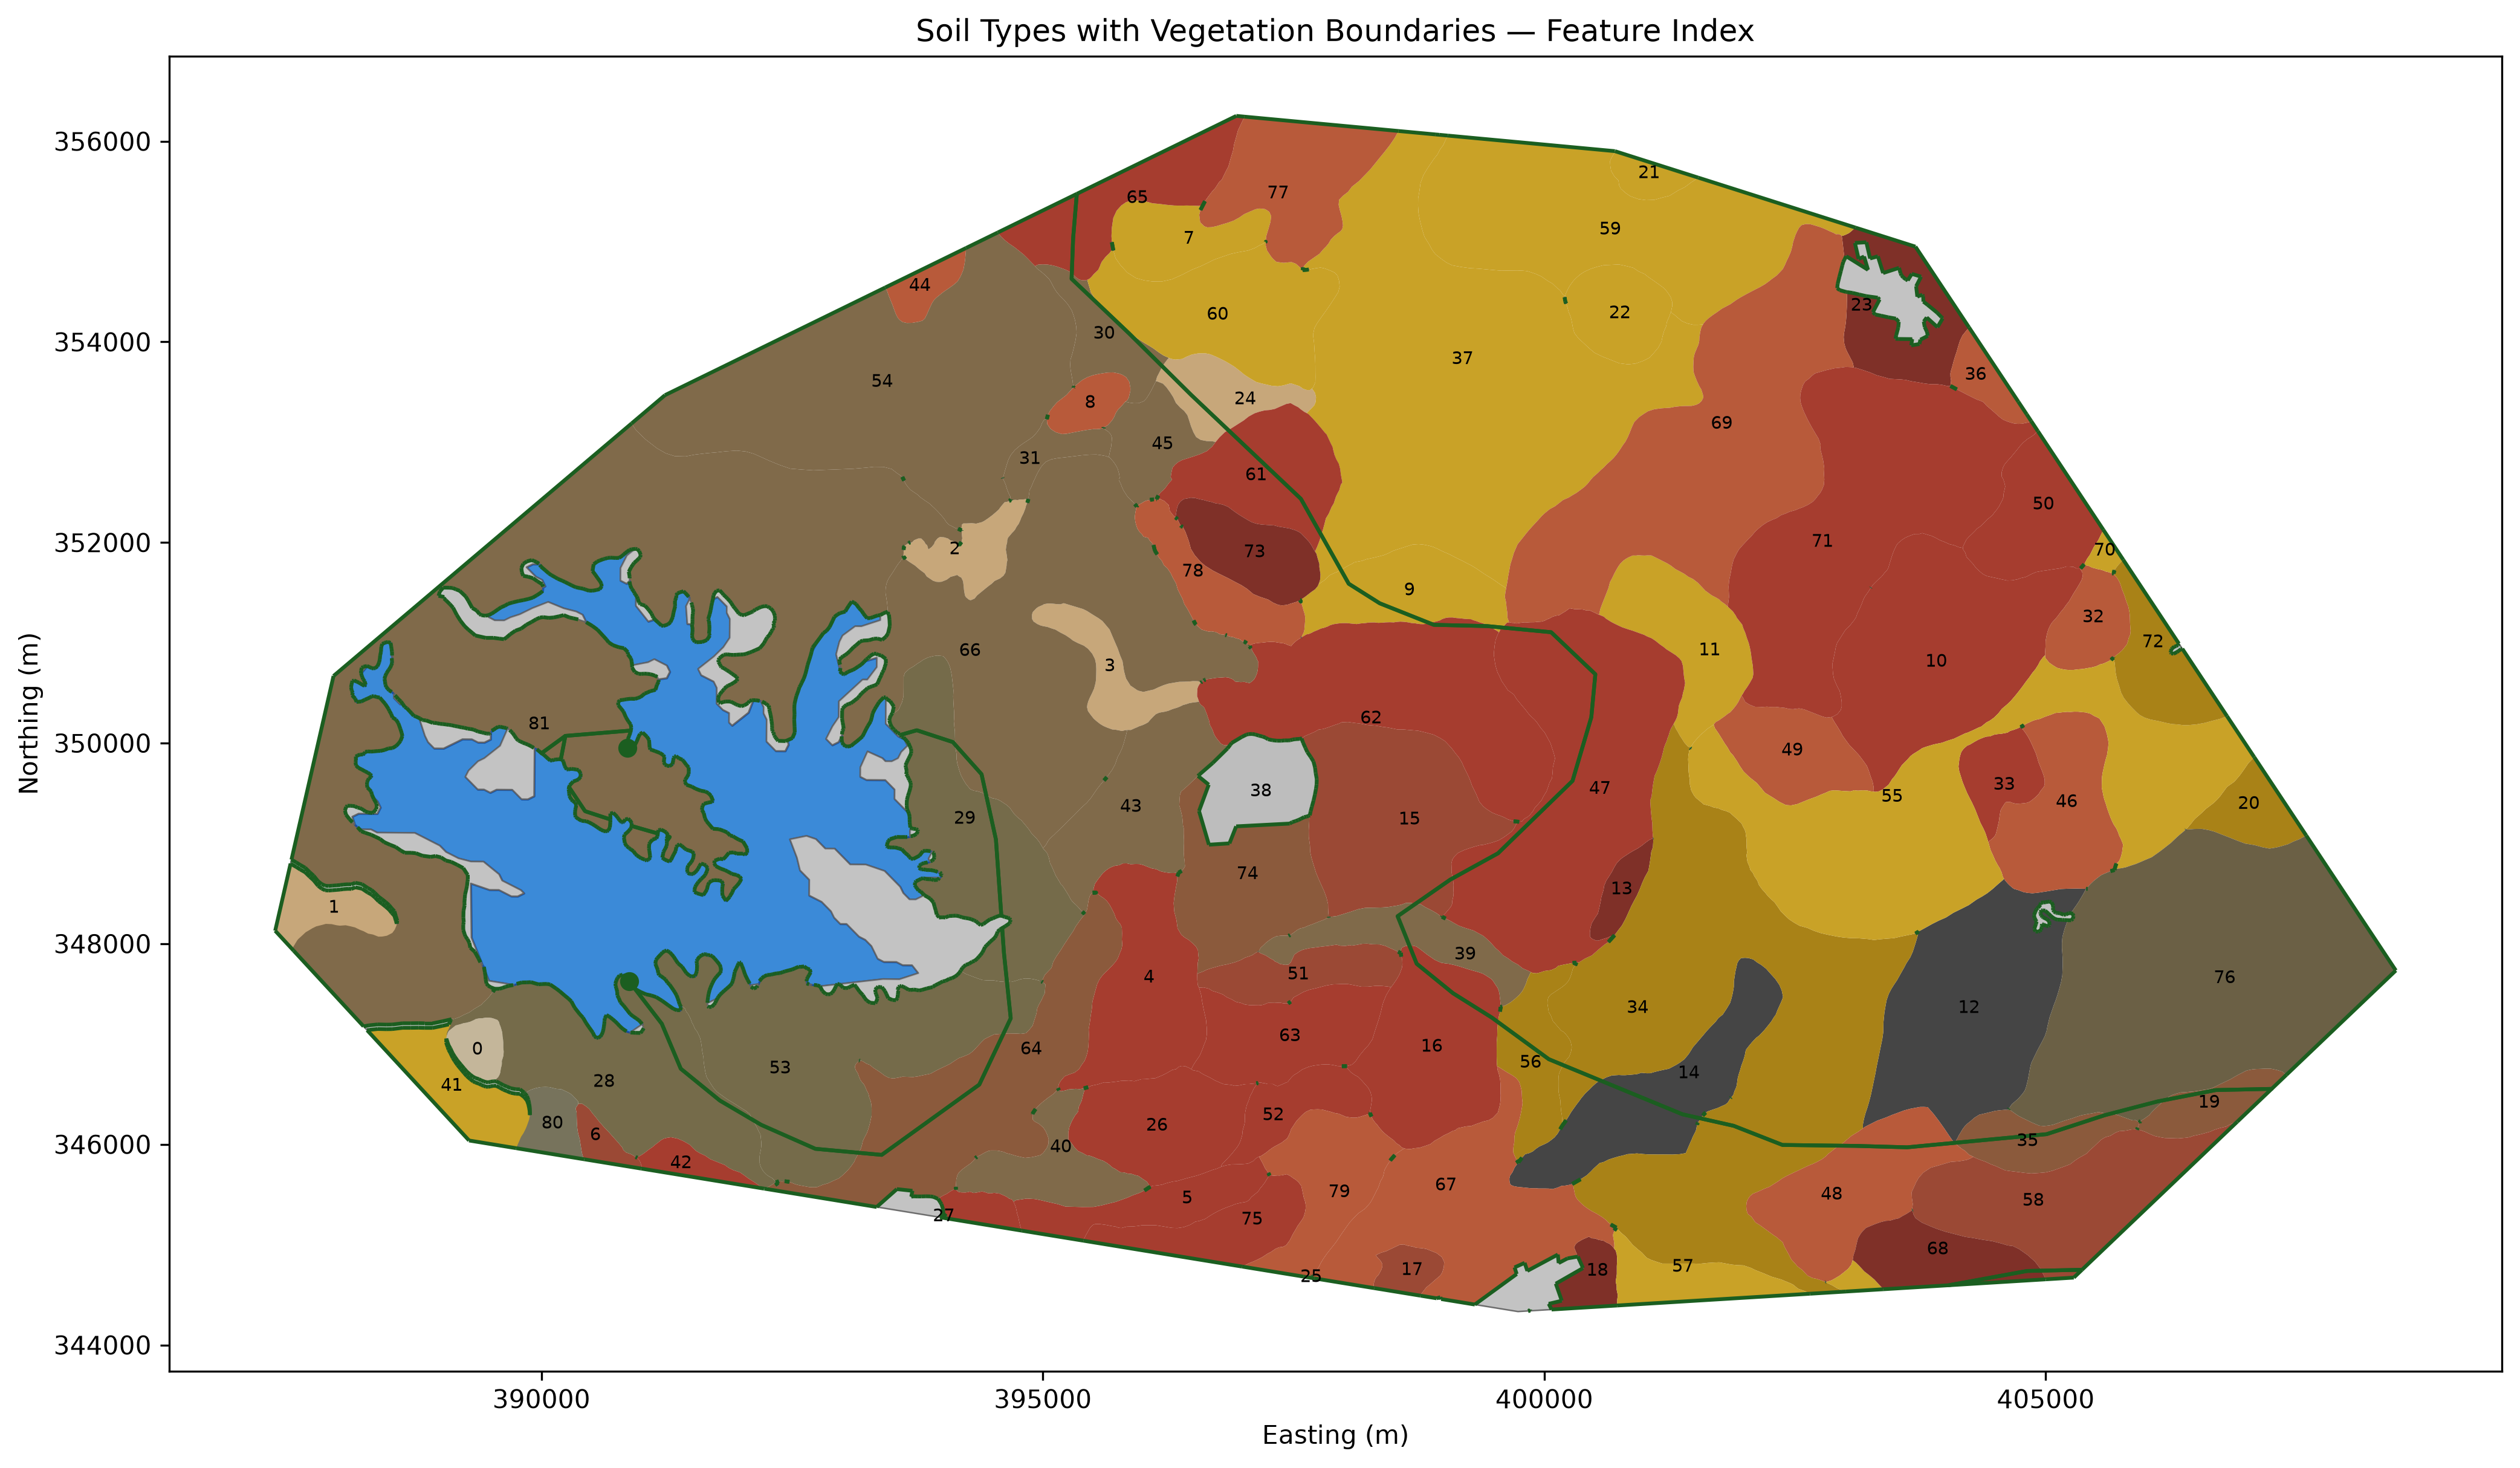
\includegraphics[
				width=\paperwidth,
				height=\paperheight
				]{soil_types_with_vegetation_boundaries.png}
			};
			
			\fill[
			forest,
			opacity=0.90
			] (current page.south west)
			rectangle (current page.north east);
			
			\node[
			align=center,
			text=white,
			text width=12cm
			] at (current page.center) {
				
				{\color{mint}\large
					OPEN-SOURCE GEOSPATIAL ANALYSIS}
				
				\vspace{0.45cm}
				
				{\fontsize{32}{36}\selectfont
					\bfseries GeoSoil-Cuba}
				
				\vspace{0.5cm}
				
				{\Large
					Soil maps. Satellite data. Spatial insight.
				}
				
				\vspace{0.8cm}
				
				{\large Ben Tamayo}
				
				\vspace{0.25cm}
				
				{\small
					Python \textbullet\ QGIS \textbullet\ GDAL
					\textbullet\ Rasterio \textbullet\ Sentinel-2
				}
				
				\vspace{0.8cm}
				
				{\color{mint}\small
					Explore the workflow, methods, and results.
				}
				
			};
			
		\end{tikzpicture}
		
	\end{frame}
	
\end{document}